% ******************************* PhD Thesis Template **************************
% Please have a look at the README.md file for info on how to use the template

\documentclass[a4paper,12pt,times,numbered, draft]{Classes/PhDThesisPSnPDF}

% ******************************************************************************
% ******************************* Class Options ********************************
% *********************** See README for more details **************************
% ******************************************************************************

% `a4paper'(The University of Cambridge PhD thesis guidelines recommends a page
% size a4 - default option) or `a5paper': A5 Paper size is also allowed as per
% the Cambridge University Engineering Deparment guidelines for PhD thesis
%
% `11pt' or `12pt'(default): Font Size 10pt is NOT recommended by the University
% guidelines
%
% `oneside' or `twoside'(default): Printing double side (twoside) or single
% side.
%
% `print': Use `print' for print version with appropriate margins and page
% layout. Leaving the options field blank will activate Online version.
%
% `index': For index at the end of the thesis
%
% `draftclassic': For draft mode without loading any images (same as draft in book)
%
% `draft': Special draft mode with line numbers, images, and water mark with
% timestamp and custom text. Position of the text can also be modified.
%
% `abstract': To generate only the title page and abstract page with
% dissertation title and name, to submit to the Student Registry
%
% `chapter`: This option enables only the specified chapter and it's references
%  Useful for review and corrections.
%
% ************************* Custom Page Margins ********************************
%
% `custommargin`: Use `custommargin' in options to activate custom page margins,
% which can be defined in the preamble.tex. Custom margin will override
% print/online margin setup.
%
% *********************** Choosing the Fonts in Class Options ******************
%
% `times' : Times font with math support. (The Cambridge University guidelines
% recommend using times)
%
% `fourier': Utopia Font with Fourier Math font (Font has to be installed)
%            It's a free font.
%
% `customfont': Use `customfont' option in the document class and load the
% package in the preamble.tex
%
% default or leave empty: `Latin Modern' font will be loaded.
%
% ********************** Choosing the Bibliography style ***********************
%
% `authoryear': For author-year citation eg., Krishna (2013)
%
% `numbered': (Default Option) For numbered and sorted citation e.g., [1,5,2]
%
% `custombib': Define your own bibliography style in the `preamble.tex' file.
%              `\RequirePackage[square, sort, numbers, authoryear]{natbib}'.
%              This can be also used to load biblatex instead of natbib
%              (See Preamble)
%
% **************************** Choosing the Page Style *************************
%
% `default (leave empty)': For Page Numbers in Header (Left Even, Right Odd) and
% Chapter Name in Header (Right Even) and Section Name (Left Odd). Blank Footer.
%
% `PageStyleI': Chapter Name next & Page Number on Even Side (Left Even).
% Section Name & Page Number in Header on Odd Side (Right Odd). Footer is empty.
%
% `PageStyleII': Chapter Name on Even Side (Left Even) in Header. Section Number
% and Section Name in Header on Odd Side (Right Odd). Page numbering in footer

% Uncomment to change page style
%\pagestyle{PageStyleII}

% ********************************** Preamble **********************************
% Preamble: Contains packages and user-defined commands and settings
% ******************************************************************************
% ****************************** Custom Margin *********************************

% Add `custommargin' in the document class options to use this section
% Set {innerside margin / outerside margin / topmargin / bottom margin}  and
% other page dimensions
\ifsetCustomMargin
  \RequirePackage[left=37mm,right=30mm,top=35mm,bottom=30mm]{geometry}
  \setFancyHdr % To apply fancy header after geometry package is loaded
\fi

% Add spaces between paragraphs
%\setlength{\parskip}{0.5em}
% Ragged bottom avoids extra whitespaces between paragraphs
\raggedbottom
% To remove the excess top spacing for enumeration, list and description
%\usepackage{enumitem}
%\setlist[enumerate,itemize,description]{topsep=0em}

% *****************************************************************************
% ******************* Fonts (like different typewriter fonts etc.)*************

% Add `customfont' in the document class option to use this section

\ifsetCustomFont
  % Set your custom font here and use `customfont' in options. Leave empty to
  % load computer modern font (default LaTeX font).
  %\RequirePackage{helvet}

  % For use with XeLaTeX
  %  \setmainfont[
  %    Path              = ./libertine/opentype/,
  %    Extension         = .otf,
  %    UprightFont = LinLibertine_R,
  %    BoldFont = LinLibertine_RZ, % Linux Libertine O Regular Semibold
  %    ItalicFont = LinLibertine_RI,
  %    BoldItalicFont = LinLibertine_RZI, % Linux Libertine O Regular Semibold Italic
  %  ]
  %  {libertine}
  %  % load font from system font
  %  \newfontfamily\libertinesystemfont{Linux Libertine O}
\fi

% *****************************************************************************
% **************************** Custom Packages ********************************

% ************************* Algorithms and Pseudocode **************************

%\usepackage{algpseudocode}


% ********************Captions and Hyperreferencing / URL **********************

% Captions: This makes captions of figures use a boldfaced small font.
%\RequirePackage[small,bf]{caption}

\RequirePackage[labelsep=space,tableposition=top]{caption}
\renewcommand{\figurename}{Fig.} %to support older versions of captions.sty


% *************************** Graphics and figures *****************************

%\usepackage{rotating}
%\usepackage{wrapfig}

% Uncomment the following two lines to force Latex to place the figure.
% Use [H] when including graphics. Note 'H' instead of 'h'
%\usepackage{float}
%\restylefloat{figure}

% Subcaption package is also available in the sty folder you can use that by
% uncommenting the following line
% This is for people stuck with older versions of texlive
%\usepackage{sty/caption/subcaption}
\usepackage{subcaption}

% ********************************** Tables ************************************
\usepackage{booktabs} % For professional looking tables
\usepackage{multirow}

%\usepackage{multicol}
%\usepackage{longtable}
%\usepackage{tabularx}


% *********************************** SI Units *********************************
\usepackage{siunitx} % use this package module for SI units


% ******************************* Line Spacing *********************************

% Choose linespacing as appropriate. Default is one-half line spacing as per the
% University guidelines

% \doublespacing
% \onehalfspacing
% \singlespacing


% ************************ Formatting / Footnote *******************************

% Don't break enumeration (etc.) across pages in an ugly manner (default 10000)
%\clubpenalty=500
%\widowpenalty=500

%\usepackage[perpage]{footmisc} %Range of footnote options


% *****************************************************************************
% *************************** Bibliography  and References ********************

%\usepackage{cleveref} %Referencing without need to explicitly state fig /table

% Add `custombib' in the document class option to use this section
\ifuseCustomBib
   \RequirePackage[square, sort, numbers, authoryear]{natbib} % CustomBib

% If you would like to use biblatex for your reference management, as opposed to the default `natbibpackage` pass the option `custombib` in the document class. Comment out the previous line to make sure you don't load the natbib package. Uncomment the following lines and specify the location of references.bib file

%\RequirePackage[backend=biber, style=numeric-comp, citestyle=numeric, sorting=nty, natbib=true]{biblatex}
%\bibliography{References/references} %Location of references.bib only for biblatex

\fi

% changes the default name `Bibliography` -> `References'
\renewcommand{\bibname}{References}


% ******************************************************************************
% ************************* User Defined Commands ******************************
% ******************************************************************************

% *********** To change the name of Table of Contents / LOF and LOT ************

%\renewcommand{\contentsname}{My Table of Contents}
%\renewcommand{\listfigurename}{My List of Figures}
%\renewcommand{\listtablename}{My List of Tables}


% ********************** TOC depth and numbering depth *************************

\setcounter{secnumdepth}{2}
\setcounter{tocdepth}{2}


% ******************************* Nomenclature *********************************

% To change the name of the Nomenclature section, uncomment the following line

%\renewcommand{\nomname}{Symbols}


% ********************************* Appendix ***********************************

% The default value of both \appendixtocname and \appendixpagename is `Appendices'. These names can all be changed via:

%\renewcommand{\appendixtocname}{List of appendices}
%\renewcommand{\appendixname}{Appndx}

% *********************** Configure Draft Mode **********************************

% Uncomment to disable figures in `draft'
%\setkeys{Gin}{draft=true}  % set draft to false to enable figures in `draft'

% These options are active only during the draft mode
% Default text is "Draft"
%\SetDraftText{DRAFT}

% Default Watermark location is top. Location (top/bottom)
%\SetDraftWMPosition{bottom}

% Draft Version - default is v1.0
%\SetDraftVersion{v1.1}

% Draft Text grayscale value (should be between 0-black and 1-white)
% Default value is 0.75
%\SetDraftGrayScale{0.8}


% ******************************** Todo Notes **********************************
%% Uncomment the following lines to have todonotes.

%\ifsetDraft
%	\usepackage[colorinlistoftodos]{todonotes}
%	\newcommand{\mynote}[1]{\todo[author=kks32,size=\small,inline,color=green!40]{#1}}
%\else
%	\newcommand{\mynote}[1]{}
%	\newcommand{\listoftodos}{}
%\fi

% Example todo: \mynote{Hey! I have a note}

% ************************ Thesis Information & Meta-data **********************
% Thesis title and author information, refernce file for biblatex
% ************************ Thesis Information & Meta-data **********************
%% The title of the thesis
\title{Accelerating the Design-Make-Test cycle of Drug Discovery with Machine Learning}
%\texorpdfstring is used for PDF metadata. Usage:
%\texorpdfstring{LaTeX_Version}{PDF Version (non-latex)} eg.,
%\texorpdfstring{$sigma$}{sigma}

%% Subtitle (Optional)
% \subtitle{that actually works}

%% The full name of the author
\author{William McCorkindale}

%% Department (eg. Department of Engineering, Maths, Physics)
\dept{Cavendish Laboratory, Department of Physics}

%% University and Crest
\university{University of Cambridge}
% Crest minimum should be 30mm.
\crest{
\includegraphics[width=0.2\textwidth]{University_Crest}}
%% Use this crest, if you are using the college crest
%% Crest long miminum should be 65mm
%\crest{
\includegraphics[width=0.45\textwidth]{University_Crest_Long}}

%% College shield [optional] 
% Crest minimum should be 30mm.
%\collegeshield{
\includegraphics[width=0.2\textwidth]{CollegeShields/Kings}}


%% Supervisor (optional)
%% for multiple supervisors, append each supervisor with the \newline command
\supervisor{Dr. Alpha Lee}

%% Supervisor Role (optional) - Supervisor (default) or advisor
% \supervisorrole{\textbf{Supervisors: }}
%% if no title is desired:
% \supervisorrole{}

%% Supervisor line width: required to align supervisors
% \supervisorlinewidth{0.35\textwidth}

%% Advisor (optional)
%% for multiple advisors, append each advisor with the \newline command
%\advisor{Dr. A. Advisor\newline
%Dr. B. Advisor}
     
%% Advisor Role (optional) - Advisor (default) or leave empty
% \advisorrole{Advisors: }
%% if no title is required
% \advisorrole{}

%% Advisor line width: required to align supervisors
%\advisorlinewidth{0.25\textwidth}


%% You can redefine the submission text:
% Default as per the University guidelines:
% ``This dissertation is submitted for the degree of''
\renewcommand{\submissiontext}{}

%% Full title of the Degree
% \degreetitle{Doctor of Philosophy}

%% College affiliation (optional)
\college{St. John's College}

%% Submission date
% Default is set as {\monthname[\the\month]\space\the\year}
%\degreedate{September 2014} 

%% Meta information
\subject{LaTeX} \keywords{{LaTeX} {PhD Thesis} {Physics} {University of
Cambridge}}


% ***************************** Abstract Separate ******************************
% To printout only the titlepage and the abstract with the PhD title and the
% author name for submission to the Student Registry, use the `abstract' option in
% the document class.

\ifdefineAbstract
 \pagestyle{empty}
 \includeonly{Declaration/declaration, Abstract/abstract}
\fi

% ***************************** Chapter Mode ***********************************
% The chapter mode allows user to only print particular chapters with references
% Title, Contents, Frontmatter are disabled by default
% Useful option to review a particular chapter or to send it to supervisior.
% To use choose `chapter' option in the document class

% ******************************** Front Matter ********************************
\begin{document}

\frontmatter

\maketitle

% % ******************************* Thesis Dedication ********************************

\begin{dedication} 

I would like to dedicate this thesis to my loving parents \dots

First and foremost, I would like to sincerely thank my advisor Alpha Lee for his help, guidance and for the freedom I was granted throughout these years.

In alphabetical order, I would also like to thank my colleagues who \dots: Dávid, Emma, Felix,  Janosh, Kadi, Penny, Rokas, Rhys.

David, Michelle, Brian. Gates scholars. CUHKPGSA?

I would finally like to warmly thank my dear housemates Dávid and Eszti for their help in moments of doubt.

WM acknowledges the support of the Gates Cambridge Trust.

\end{dedication}
% ******************************* Thesis Declaration ***************************

\begin{declaration}

I hereby declare that except where specific reference is made to the work of others, the contents of this dissertation are original and have not been submitted in whole or in part for consideration for any other degree or qualification in this, or any other university. This dissertation is my own work and contains nothing which is the outcome of work done in collaboration with others, except as specified in the Preface and Acknowledgements. This  dissertation contains fewer than 65,000 words including appendices,  bibliography, footnotes, tables and equations and has fewer than 150 figures.

The research described in this thesis was performed between October 2019 and December 2022, and was supervised by Dr Alpha A. Lee.
% Author and date will be inserted automatically from thesis.tex \author \degreedate

\end{declaration}
% ************************** Thesis Acknowledgements **************************

\begin{acknowledgements}

TODO - finish acknowledgements

First and foremost, I would like to sincerely thank my supervisor Dr Alpha A. Lee for his invaluable guidance, support, and encouragement throughout my PhD journey. I am deeply grateful for his commitment to my success and for his role in shaping my personal and professional development.

In alphabetical order, I would also like to thank my colleagues in the Lee Group: Dávid, Emma, Felix, Janosh, Kadi, Penny, Rokas, Rhys. Their knowledge, expertise, and friendship have been invaluable in shaping my research and personal growth. I feel very fortunate to have had the opportunity to work with and learn from you all, and I will always cherish the memories and lessons learned from our time together.

I was generously funded by the Gates Cambridge Scholarship to undertake this research, and I am very grateful for their support, as well as for the many friendships I have made in the Gates scholar community. I would like to give special thanks in particular to David and Michelle, for their friendship and support.

Friends from Cambridge. Brian.

Upheaval in my birthplace, Hong Kong. CUHKPGSA

Much of the research in this thesis was conducted during the COVID-19 pandemic, when I spent a considerable amount of time indoors with my dear housemates Dávid and Eszti. I will be forever grateful for their unwavering friendship, humor, and kindness during some of the most challenging times of my PhD journey.

I would like to thank Marika for always putting a smile on my face and reminding me what is truly important in life.

Lastly, I would like to thank my parents, John and Maureen, for their unconditional love and continual support.

\end{acknowledgements}

% ************************** Thesis Abstract *****************************
% Use `abstract' as an option in the document class to print only the titlepage and the abstract.
\begin{abstract}
Drug discovery follows a design-make-test cycle of proposing drug compounds, synthesising them, and measuring their bioactivity, which informs the next cycle of compound designs. The challenges associated with each step leads to the long timeline of preclinical pharmaceutical development. This thesis focuses on how we can use machine learning tools to accelerate the design-make-test cycle for faster drug discovery.

We begin with the design of new compounds, looking at the initial stage of fragment-based hit finding where only the 3D coordinates of fragment-protein complexes are available. The standard approach is to “grow” or “merge” nearby fragments based on their binding modes, but fragments typically have low affinity so the road to potency is often long and fraught with false starts. Instead, we can reframe fragment-based hit discovery as a denoising problem - identifying significant pharmacophore distributions from an “ensemble” of fragments amid noise due to weak binders - and employ an unsupervised machine learning method to tackle this problem. We construct a model that screens potential molecules by evaluating whether they recapitulate those fragment-derived pharmacophore distributions. We show that this approach outperforms docking on distinguishing active compounds from inactive ones on historical data. Further, we prospectively find novel hits for SARS-CoV-2 Mpro and the Mac1 domain of SARS-CoV-2 non-structural protein 3 by screening a library of 1B molecules.

After identifying hit compounds, we enter the the hit-to-lead stage where we wish to optimise their molecular structures to improve bioactivity. Framing bioactivity modelling as classification of active/inactive would not allow us to rank compounds based on predicted bioactivity improvement, while the low number of active compounds and the measurement noise make a regression approach challenging. We overcome this challenge with a learning-to-rank framework via a classifier that predicts whether a compound is more or less active than another using the difference in molecular descriptors between the molecules as input. This allows us to make use of inactive data, and threshold the bioactivity differences above measurement noise. Validation on retrospective data for Mpro shows that we can outperform docking on ranking ligands, and we prospectively screen a library of 8.8M molecules and arrive at a potent compound with a novel scaffold.

After designing a drug candidate one needs to find a synthesis route to actually make the molecule in the real world. An exciting approach is to use deep learning models trained on patent reaction databases, but they suffer from being opaque black-boxes. It is neither clear if the models are making correct predictions because they inferred the salient chemistry, nor is it clear which training data they are relying on to reach a prediction. To address this issue, we developed a workflow for quantitatively interpreting a state-of-the-art deep learning model for reaction prediction. By analysing chemically selective reactions, we show examples of correct reasoning by the model, explain counterintuitive predictions, and identify Clever Hans predictions where the correct answer is reached for the wrong reason due to dataset bias.

Testing a drug candidate typically involves obtaining a pure sample of the molecule, and then measuring its bioactivity in solution via an assay. While necessary for maximum accuracy, compound purification can be time-consuming and costly. We investigated whether we needed compound purification at all for training machine learning bioactivity models by assaying crude reaction mixtures instead of pure samples. This approach allowed us to obtain bioactivity data in higher throughput and train useful models for identification of false negative assay measurements, as well as prospective screens.

The research presented in this thesis highlights the promise of applying machine learning in accelerating the design-make-test cycle of drug discovery. This thesis concludes by outlining promising research directions for applying machine learning within drug discovery.
\end{abstract}


% *********************** Adding TOC and List of Figures ***********************

\tableofcontents

% \listoffigures

% \listoftables

% \printnomenclature[space] space can be set as 2em between symbol and description
%\printnomenclature[3em]

% \printnomenclature

% ******************************** Main Matter *********************************
\mainmatter

% TODO - update chapter names
\chapter*{Preface}
\addcontentsline{toc}{chapter}{Preface}
\hyperref[ch:intro]{Chapter 1} introduces the design-make-test cycle in drug discovery and the promise of machine learning (ML) for accelerating the process.

\hyperref[ch:background]{Chapter 2} gives an overview of molecular featurisation and computational methods which are used in this thesis. COVID Moonshot, a drug discovery inititative that much of this thesis is based on, is also introduced.

In \hyperref[ch:fresco]{Chapter 3} starts at the hit-finding stage of drug discovery, and we discuss the usage of unsupervised learning for modelling the 3D distribution of pharmacophores in fragment-protein complexes. This work resulted in the following preprint (manuscript under review):
\begin{quote}
William McCorkindale, Ivan Ahel, Haim Barr, Galen J. Correy, James S. Fraser, Nir London, Marion Schuller, Khriesto Shurrush, Alpha A. Lee. Fragment-Based Hit Discovery via Unsupervised Learning of Fragment-Protein Complexes.
\end{quote}
In this work, I implemented the model and conducted the computational validation and virtual screening. Dr Ivan Ahel, Dr Haim Barr, Dr Khriesto Shurrush, and Prof Nir London performed bioactivity assays of ligands against SARS-CoV-2 Mpro. Dr Galen Correy and Prof James Fraser obtained X-ray crystallographic structures of ligand-bound structures to SARS-CoV-2 nsp3-Mac1. Dr Marion Schuller performed bioactivity assays of ligands against nsp3-Mac1. Dr Alpha A. Lee supervised the work.

\hyperref[ch:ranking]{Chapter 4} brings us to the hit-to-lead stage where modelling bioactivity becomes possible, and we discuss using a model that learns to rank molecules pairwise by activity. This work resulted in the following publication:
\begin{quote}
Aaron Morris, William McCorkindale, The COVID Moonshot Consortium, Nir Drayman, John D. Chodera, Savaş Tay, Nir London, and Alpha A. Lee. Discovery of SARS-CoV-2 main protease inhibitors using a synthesis-directed de novo design model, \textit{Chem. Commun.}, 2021,57, 5909-5912 
\end{quote}
In this work, I developed the ranking model and constructed the screening library. Aaron Morris evaluated the model and generated compound synthesis routes. Dr John D. Chodera performed docking calculations. Prof Nir London performed bioactivity assays of ligands against SARS-CoV-2 Mpro. Dr Nir Drayman and Prof Savaş Tay performed OC43 live virus assays. Dr Alpha A. Lee supervised the work.

In \hyperref[ch:transformer]{Chapter 5} we quantitatively explain predictions from deep learning models used for chemical reactions prediction, revealing model biases due to shortcomings in the training data. This work resulted in the following publication:
\begin{quote}
Dávid Péter Kovács, William McCorkindale and Alpha A. Lee. Quantitative interpretation explains machine learning models for chemical reaction prediction and uncovers bias. \textit{Nature Communications} volume 12, Article number: 1695 (2021)
\end{quote}
I worked jointly with Dávid Kovács on this work which he completed as part of his MPhil research project under Dr Alpha A. Lee. We contributed equally to model development. Dávid Kovács trained the models and analysed the model attributions for various reaction classes. I applied reaction templates for data analysis and artificial dataset generation and investigated model performance under Tanimoto splitting. Dr Alpha A. Lee supervised the work.

\hyperref[ch:testing]{Chapter 6} discusses the training of ML models on high-throughput bioactivity measurements from crude reaction mixtures instead of purified compounds. This research was carried out in collaboration with Dr Emma King-Smith, Mihajlo Filep, Prof Nir London, and Dr Alpha A. Lee. In this work, I implemented the random forest model and constructed the screening library. Dr Emma King-Smith implemented the gaussian process model and cleaned the experimental data. Mihajlo Filep performed bioactivity assays against SARS-CoV-2 Mpro. Dr Alpha A. Lee and Prof Nir London supervised the work.

The final chapter summarises the research presented and discusses promising directions for future research.

During the course of this thesis, several fruitful collaborations have also led to the following publications. These are not discussed in detail within this dissertation.

\begin{quote}
 Kadi L. Saar, William McCorkindale, Daren Fearon, Melissa Boby, Haim Barr, Amir Ben-Shmuel, The COVID Moonshot Consortium, Nir London, Frank von Delft, John D. Chodera and Alpha A. Lee. Turning high-throughput structural biology into predictive inhibitor design. \textit{Proceedings of the National Academy of Sciences} volume 120 (11), Article number: e2214168120 (2023)
\end{quote}

\begin{quote}
 Ryan-Rhys Griffiths, Jake L Greenfield, Aditya R Thawani, Arian R Jamasb, Henry B Moss, Anthony Bourached, Penelope Jones, William McCorkindale, Alexander A Aldrick, Matthew J Fuchter, and Alpha A. Lee. Data-driven discovery of molecular photoswitches with multioutput Gaussian processes. \textit{Chemical Science} volume 13 (45), Article number: 13541-13551 (2022)
\end{quote}
%!TEX root = ../thesis.tex
%*******************************************************************************
%****************************** Third Chapter **********************************
%*******************************************************************************
\chapter{Introduction}
The discovery of new pharmaceuticals traditionally follows the design-make-test paradigm, where molecules are repeatedly proposed, synthesized, and assayed. Drug candidates are designed based on some hypothesis relating chemical structure to drug activity, which gets updated in light of new activity results. This cycle repeats as the molecular search space narrows down until a candidate molecule satisfies the necessary activity/selectivity/toxicity criteria.

\begin{figure}[!h] % !h ~ force here, t ~ top, b ~ bottom, p ~ separate page
\centering
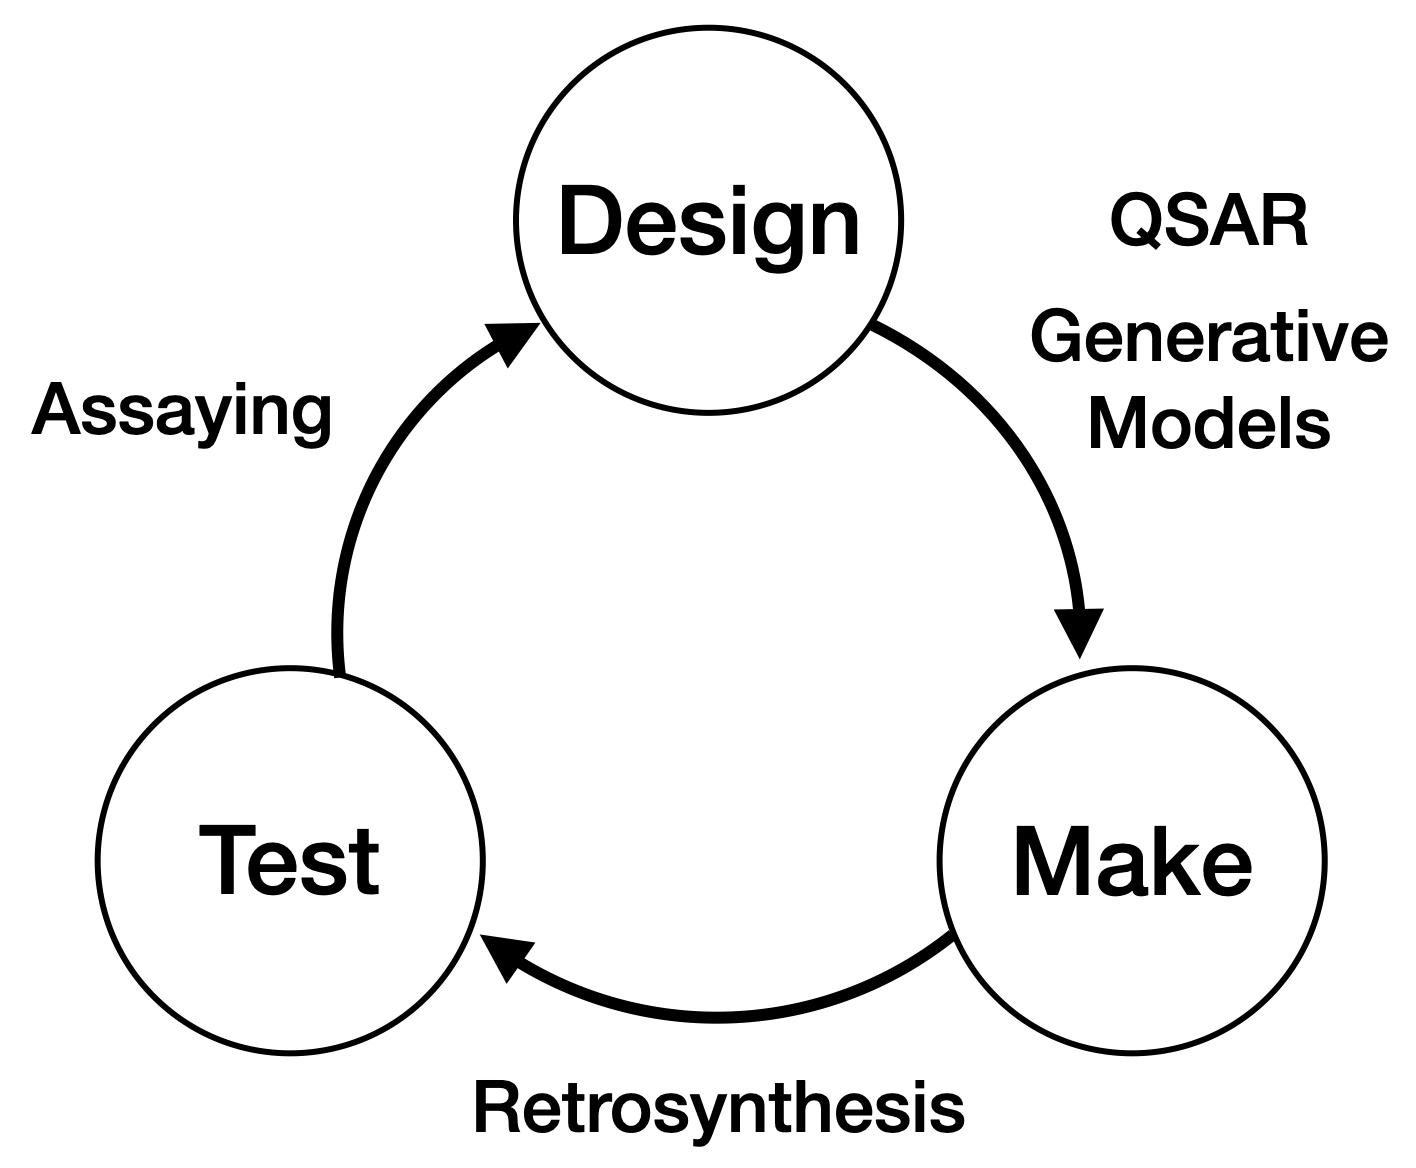
\includegraphics[width=0.5\textwidth]{Ch1/Figs/design-make-test.png}
\caption{\label{fig:cycle} An overview of the design-make-test cycle in drug discovery.}
\end{figure}

While computational methods have long been used in various stages of the cycle, there has been a recent surge in applying artificial intelligence to drug discovery following its success in various other fields, most notably computer vision and natural language processing. Since molecular assaying is largely an automated process the application focus has been on `design' and `make' \cite{Coley2019AutonomousProgress}, for example in modelling quantitative structure-activity relationships (QSAR), designing generative models for proposing drug candidates, and planning retrosynthesis routes (Fig~\ref{fig:cycle}). 

As the field of data-driven drug discovery matures beyond merely adapting the latest state-of-the-art machine learning (ML) methods, the present challenge is to tailor ML models specifically for the unique problems and situations faced in pharmaceutical chemistry. This report summarizes my efforts over the past year to play a part in this challenge with intuitions based on physical science. These consist of three separate tasks, one on `Make' and two on `Design':

\begin{itemize}
    \item \textbf{Interpreting learnt chemical principles from Molecular Transformer:} a state-of-the-art reaction prediction model (Molecular Transformer) was investigated with input and data attribution methods to discern whether the model had learnt chemically reasonable patterns of reactivity, or had simply succumbed to hidden bias in the datasets.
    \item \textbf{Exploiting molecular shape for property prediction:} a descriptor of atomic positions known as SOAP, which has seen widespread use in condensed matter physics due to its symmetry-invariance properties, was utilized in a Gaussian Processes model and shown to be competitive with other state-of-the-art models on predicting bioactivity. It was also demonstrated that ensembling models with diverse representations led to further predictive power.
    \item \textbf{Designing Sars-CoV-2 MPro inhibitors:} An initiative known as COVID Moonshot \cite{moonshot2020} was established to search for inhibitors of the Sars-CoV-2 main protease (MPro), crowd-sourcing drug candidate designs from the scientific community. In the early stages of the project, I utilised a genetic algorithm with SOAP descriptors for combining disparate fragment hits; in the most recent stage, I implemented a graph siamese network to learn how to rank the activity of assayed molecules, which was then used to suggest new candidates via computational screening of a constructed library.
\end{itemize}
The lessons learnt from these projects are used to inform possible avenues of future research, which are discussed in the final chapter of this report.

\chapter{Fragment-Based Hit Discovery via Unsupervised Learning of Fragment-Protein Complexes}
In this work, we describe an end-to-end hit detection approach that bridges the the paradigms of both fragment-based drug design and virtual screening. Our method, named FRESCO, utilises unsupervised learning to learn pharmacophore distributions directly from experimental 3D fragment-protein structures. The trained model evaluates whether or not a particular compound possesses pharmacophores matching the distribution exhibited by the bound fragments, replicating the intuition of a medicinal chemist deducing spatial correlations between pharmacophores from different fragments. Our approach is computationally validated with a retrospective study on SARS-CoV-2 main protease (Mpro) ligands using data from COVID Moonshot \cite{Moonshot2022}, showing high enrichment. Then, we conduct an experimental search for novel hits for Mpro and the Mac1 domain of SARS-CoV-2 non-structural protein 3 (nsp3) by scoring a library of 1.4 billion purchasable compounds from EnamineREAL, resulting in 1 (novel?) hit for MPro and 2 (novel?) hits for Mac-1. (Scaffold exploration of the detected hits hopefully lead to novel potent ligands!) Our results are the first experimentally validated demonstration of hit detection via a fully computational workflow starting directly from an experimental fragment screen.

\section{Introduction}

TODO - shorten introduction, put some of it in discussion?

Developing a new drug from original idea to the launch of a finished product is a complex process which can take 12–15 years and cost in excess of \$1 billion \cite{Hughes2011Principles}. A key step in the early stages of the drug discovery process following the identification of a biological target is hit detection. Broadly speaking, a `hit' is a compound that interacts with the identified target sufficiently strong enough to act as a starting point for optimisation of the compound structure towards a candidate drug. 

Approaches towards hit detection generally involve the screening of libraries of compounds. For example, in high throughput screening (HTS) often hundreds of thousands of chemical compounds are synthesised and tested, requiring substantial resources as well as complex logistics. While experimental techniques such as DNA-Encoded libraries are being developed to increase the efficiency of large-scale compound screening \cite{GirondaMartinez2021DNALibrary}, there has been a growing push towards conducting hit detection computationally instead to decrease the cost and accelerate this step of the drug discovery process \cite{?}. 

In this approach, known as virtual screening, a computational scoring function is used to estimate the potency of a compound. After computing the scores for all of the compounds in a library, only those ranked highly by the scoring function are chosen for synthesis and experimental validation. Currently the predominant scoring function used to conduct a virtual screen is molecular docking. In molecular docking, the 3D conformation of a ligand and the target are explicitly modelled and a physics-based simulation of the binding process is conducted, with the calculated energy of the bound ligand as the score. Although this approach has yielded success \cite{Lyu2019UltraLargeDocking,Alon2021SigmaTwo}, correctly performing molecular docking is non-trivial and the deficiencies of molecular docking for bioactivity prediction are well-documented \cite{Llanos2021StrengthsAndWeaknesses, Macip2022HasteMakesWaste}.


\begin{figure}
    \centering
    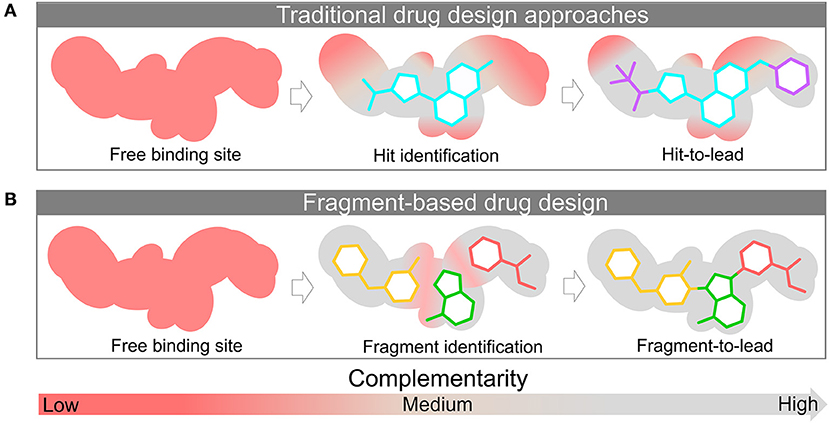
\includegraphics[width=\linewidth]{Ch2/Figs/fbdd_vs_trad.jpg}
    \caption{An illustration comparing fragment-based drug discovery to traditional approaches.}
    \label{fig:fbdd}
\end{figure}

An alternative to these methodologies is fragment-based drug discovery (FBDD). In this approach, a library of very low molecular weight compounds (`fragments' typically less than 18 nonhydrogen atoms \cite{David2017FBLD}) are screened at high concentrations alongside the generation of bound fragment-protein structures via X-ray crystallography or cryo-EM. By obtaining these experimental structures and examining the binding interactions between individual fragments with protein residues, fragments can be used as building blocks for larger molecules by linking or merging together disparate fragments in order to increase potency. Conceptually, FBDD is based on a coarse-graining of fragments to specific moieties or groups that are associated with interactions to the target, with the goal of maintaining and optimising these interactions in larger molecules.

 Although there exist some computational approaches for supporting FBDD, for example hot spot analysis and pocket druggability prediction \cite{deSouza2020InSilicoFBDD}, at present the main procedure of selecting which fragments to merge and how to do so remains largely intuition-based and human-driven. (and fraught to error? citation needed \cite{?})

In this work, we describe an end-to-end hit detection approach that bridges the the paradigms of both fragment-based drug design and virtual screening. Our method, named FRESCO, utilises unsupervised machine learning to learn pharmacophore distributions directly from experimental 3D fragment-protein structures. The trained model acts as a scoring function that can be used to perform virtual screening, evaluating whether or not a particular compound possesses pharmacophores matching the distribution exhibited by the bound fragments. 

This methodology aims to replicate the intuition of a medicinal chemist preforming fragment-based drug discovery, abstracting fragments to pharmacophores and deducing spatial correlations between pharmacophores from different fragments. As a matter of fact, we go beyond the typical strategem of growing one individual fragment independently of the others, or merging two particular fragments - by training our model on all of the fragment-protein structures we leverage information from all existing fragments, ensuring no pharmacophore correlations are overlooked in the hit detection process.

We first computationally validate our approach with a retrospective study on bioactivity prediction for SARS-CoV-2 main protease (Mpro) ligands using data from COVID Moonshot \cite{Moonshot2022}, showing high enrichment. Then, we conduct an experimental search for novel hits for Mpro and the Mac1 domain of SARS-CoV-2 non-structural protein 3 (nsp3) by performing a virtual screen with FRESCO on a library of 1.4 billion purchasable compounds from EnamineREAL. This resulted in 1 (novel?) hit for MPro and 2 (novel?) hits for Mac-1, with crystallographic poses for the Mac-1 hits. Follow-up compounds for performing scaffold exploration of the detected hits were synthesised and assayed demonstrating credible structure-activity relationships, confirming that the detected hits were genuine.

Our method is unique not only in its philosophy, but also its use of unsupervised learning in the form of kernel density estimation. Although there has been a rapid growth in machine learning methods applied to drug discovery in recent years particularly in QSAR/molecular property prediction, the vast majority of them are supervised learning techniques requiring not merely the existence of experimental assay data, but its existence in sufficient quantity and quality to train a useful model. The nature of the problem of hit detection in early-stage drug discovery is one where such data in nonexistent, which underlies the necessity of having methods for directly performing hit detection from fragment screen data. 

The only comparable methods that the authors are aware of is recent work in using deep generative models for proposing merges between two fragments (DeLinker \cite{Imrie2020DeLinker}, SyntaLinker \cite{Yang2020SyntaLinker}, and Develop \cite{Imrie2021Develop}). These approaches differ for ours in several ways: Firstly, these models all require human intervention from an expert in choosing which fragments to merge, or what pharmacophoric constraints need to obeyed, whereas our model is fully end-to-end. Secondly, these methods utilise neural network-based generative models which are very sensitive to training hyperparameter choice in general (citation about mode collapse \cite{?}), and for molecular generation in particular known to propose invalid and/or unsynthesizable molecules \cite{Gao2020Synthesizability}. In contrast, our method relies on kernel density estimation which is simple, robust and free from hyperparametear tuning, and we we explicitly only screen purchasable, easily-synthesised molecules. Lastly, the proposed models have only been studied computationally and lack validation in the real world.

Our results are the first experimentally validated demonstration of hit detection via a fully computational workflow starting directly from an experimental fragment screen. This work opens the door for bridging fragment-based drug discovery with virtual screening.

\section{Results}


\subsection{Computational Retrospective Study}

To validate that our hypothesised methodology has merit, a computational study was conducted on the SARS-CoV-2 main protease (Mpro). The COVID Moonshot campaign \cite{Moonshot2022} was established as an open science effort towards developing a patent-free antiviral drug for the SARS-CoV-2, specifically targeting the inhibition of Mpro as that would prevent the virus from further replication. Throughout the campaign, activity data consisting of the structures of molecules that were synthesised and assayed was continually released. As a proof-of-concept, the model predictions for the assayed molecules are compared against the measured activity and analysed.

Firstly, the FRESCO model was fit on publicly reported crystallographic structures of non-covalent fragments bound to the SARS-CoV-2 Mpro protein \cite{Douangamath2020XChem}. Next, conformer coordinates for Moonshot compounds reported before March 22nd 2021 were obtained from parallel work within the Moonshot consortium performing docking studies on Mpro (TODO - citation/explanation?). Pharmacophore features were generated from these conformers and the molecules were scored using the model. The enrichment factor for picking compounds above an IC50 of 10\uM is computed as we are most interested in the ability of this model to sample potent compounds. We also compute the enrichment from ranking the compounds with the Chemgauss4 scoring function.

\begin{figure}
    \centering
    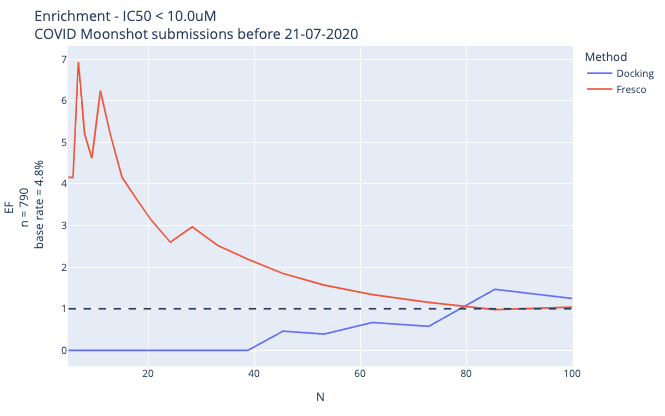
\includegraphics[width=\textwidth]{Ch2/Figs/enrichment_vs_docking.png}
    \caption{FRESCO is able to detect potent compounds purely based on unsupervised learning. High enrichment relative to docking is achieved when performing a retrospective study on activity data COVID Moonshot.}
    \label{fig:moonshot_enrichment_vs_docking}
\end{figure}

The results are shown in Fig. \ref{fig:moonshot_enrichment_vs_docking} illustrating high enrichment, validating the hypothesis that it is possible to correlate bioactivity with unsupervised learning of fragment pharmacophore distributions. The date 21st July 2021 marks when additional experimental data was released and the direction of the COVID Moonshot campaign shifted from hit detection to optimisation of existing lead compounds \cite{Moonshot2021DataRelease}. The optimisation process relies on the improvement of energetic interactions between the ligand and residues in the active site, likely growing beyond the volume covered by the initial fragment hits and so cannot in principle be captured by FRESCO. This is consistent with the observed decrease in enrichment relative to docking when using data from latter stages of Moonshot where more of the submitted compounds are designed for reaching nanomolar affinity. This shows the value in using FRESCO for hit detection in the early stages of a drug discovery campaign.

TODO - Which enrichment curves to show? Put some in the SI? Should I include ZINC graph?

\subsection{Experimental Prospective Study}
After confirming the merit of this approach via a retrospective computational study, a prospective experimental search for novel hits was performed to demonstrate the capability of this methodology. We study two targets: the main protease (Mpro) of SARS-CoV-2 and the Mac1 domain of SARS-CoV-2 non-structural protein 3 (nsp3). 

For both targets we followed the same workflow to discover novel hits. We first fit FRESCO models on experimental fragment-protein crystal complexes, and used the models to screen the VirtualFlow \cite{Gorgulla2020VirtualFlow} library of commercially available compounds. The top predicted compounds were filtered by their physical properties and were clustered by structural similarity. The centroids of the 50 most populous clusters were selected as hit candidates and ordered for synthesis and testing. Details on the methodology can be found in Sec. \ref{sec:methods}.

\subsubsection{Mpro}
For Mpro, 38 compounds were successfully synthesised and assayed. One of the compounds, WIL-UNI-d4749f31-37, was recorded with an IC50 of 25.8\uM measured via fluorescence assay while the remaining compounds were found to be inactive. To confirm that the compound activity was not a false positive (eg measured potency due to assay interference) and that genuine ligand-protein interactions existed, a follow-up series of 8 compounds (ALP-UNI-ed5cdfd2) consisting of structural perturbations to the molecular scaffold was also synthesised and assayed. All 8 compounds exhibited inhibition at high concentrations and one compound (ALP-UNI-ed5cdfd2-1) had a lower IC50 of 19.4\uM, demonstrating a genuine structure–activity relationship SAR for this hit compound.

Mpro order 1st batch = WIL-UNI-d4749f31, order 2nd batch = WIL-UNI-2a57d06c (no actives). 

\begin{figure}
    \centering
    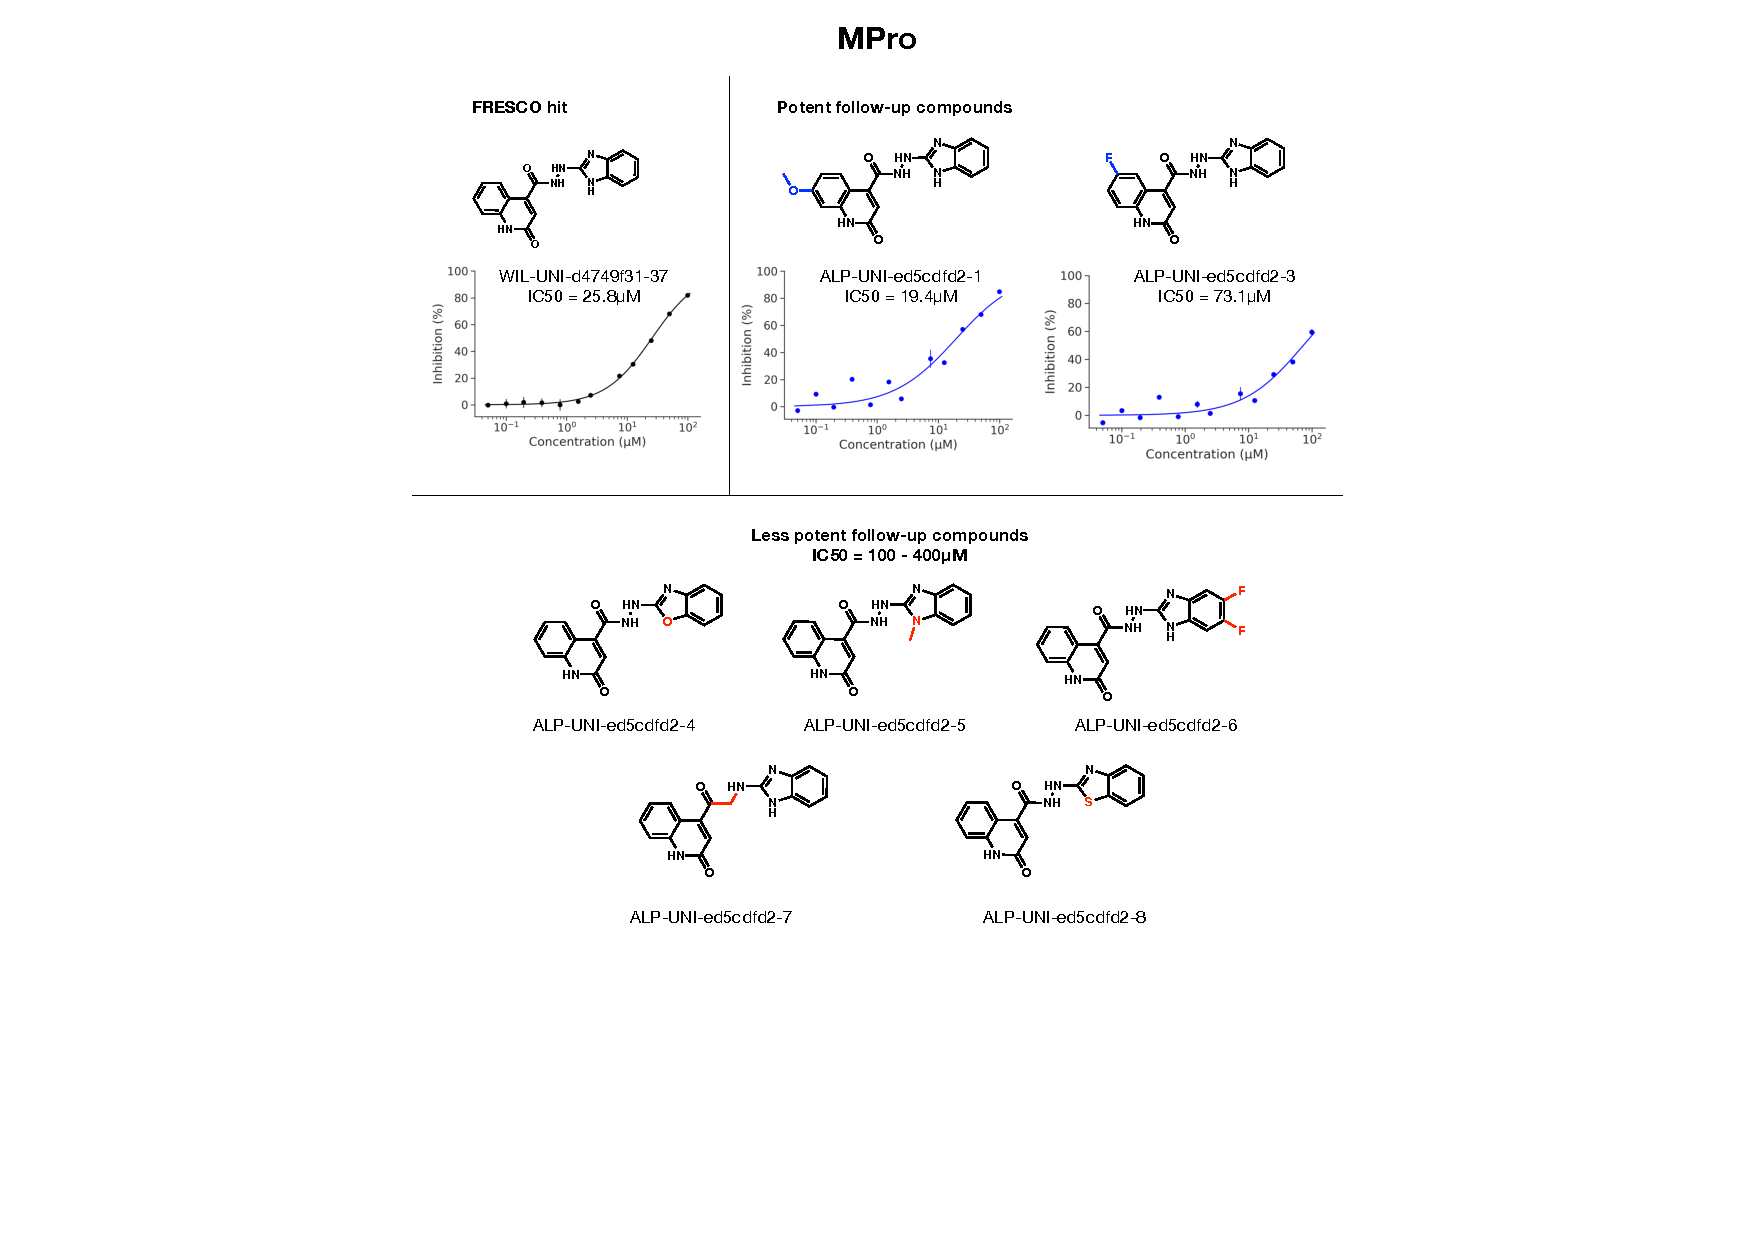
\includegraphics[width=\linewidth]{Ch2/Figs/mpro_hit_IC50.png}
    \caption{Dose-Response curve for WIL-UNI-d4749f31-37 and follow-up compounds demonstrating SAR relationship.}
    \label{fig:mpro_hit}
\end{figure}

\subsubsection{Mac-1}
For Mac-1, 52 compounds were successfully synthesised and assayed. Two of the compounds show non-negligible activity at high concentration - at 250\uM, compound Z5551425673 (as a racemic mixture) has an inhibition of 30.1\% , while compound Z1102995175 has 24.8\%. In addition, crystallographic structures of Z5551425673 (modelled as the S-stereoisomer) bound to the active site was also found alongside that of 3 other compounds (Z2890189003, Z2890182452, Z1423250928), confirming that Z5551425673 is a true hit.

As with Mpro, a follow-up series of compounds were designed to perturb the chemical structure of Z5551425673 in order to confirm the existence of SAR for this compound against Mac-1. 26 compounds were ordered and ... TODO.

\begin{figure}
    \centering
    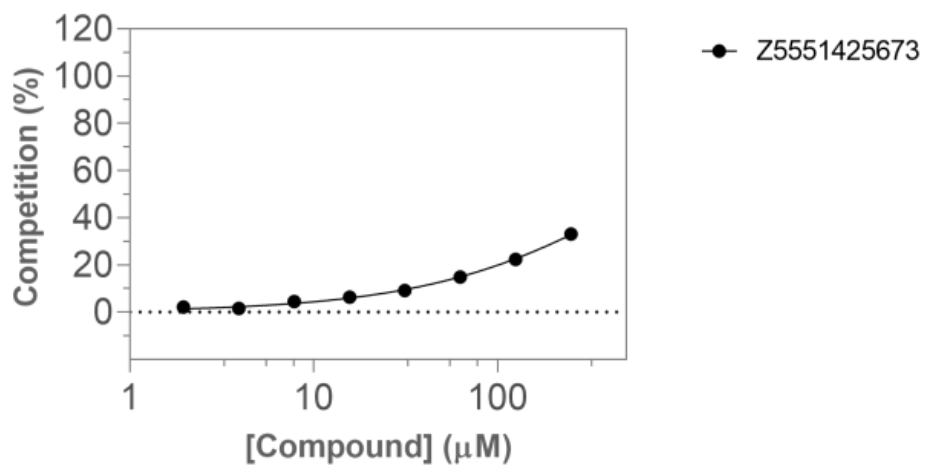
\includegraphics[width=\linewidth]{Ch2/Figs/mac1_hit_IC50.png}
    \caption{Dose-Response curve for Z5551425673 and follow-up compounds demonstrating SAR relationship. Also showing crystal structure TODO.}
    \label{fig:mac1_hit}
\end{figure}

TODO - table and structures in SI

\section{Discussion}

TODO - improvements that could be made? Future extensions? Transfer learning between targets? Docked fragments? Ensemble dock scores with FRESCO scores?

\section{Conclusion}

\section{Methods} \label{sec:methods}
\subsection{Datasets}

The crystal structures were downloaded from \href{https://fragalysis.diamond.ac.uk/viewer/react/landing}{\texttt{Fragalysis}}. For Mpro, non-covalent fragments from the XChem fragment screen \cite{Douangamath2020XChem} were used while for Mac-1 both XChem and UCSF fragment data were used.

The Moonshot activity data for the retrospective study was accessed in Mar 22nd 2021. The IC50 values in that dataset, as well as in the prospective study on Mpro were measured from a fluorescence based enzyme activity assay.

For Virtual Screening, we utilize a published dataset of more than 1.4 billion commercially available molecules from EnamineREAL \& ZINC15 in a ready-to-dock format \cite{Gorgulla2020VirtualFlow}.

\subsection{Model Construction}
The model used in this work takes as input the 3D pharmacophore distribution of a candidate molecule, and evaluates the log-probability that the distribution matches that of the fragment screen on the target site.

The 3D pharmacophore distribution of a molecule is obtained by extracting pharmacophores from the molecular SMILES and their corresponding conformer coordinates, and then evaluating the pairwise distance matrix between all possible pharmacophore pairs (eg Donor-Donor \& Aromatic-Acceptor). SMARTS pattern matching following default pharmacophore definitions in \href{https://www.rdkit.org/docs/index.html}{\texttt{RDKit}} were used to extract pharmacophores from the fragment SMILES. The pharmacophores considered are hydrogen bond donors, hydrogen bond acceptors, and aromatic rings. The coordinates of each pharmacophore are defined as the average over the atoms in the pharmacophore (eg the position of an aromatic pharmacophore from a benzene ring would be the mean of the coordinates of the 6 carbon atoms in the ring). 

For some fragments, multiple crystallographic poses are recorded. To account for this, we weigh the contribution of each fragment structure to the overall fragment pharmacophore distribution by $\frac{1}{n}$ where $n$ is the number of conformations recorded for each conformer. In addition, we exclude the counting of correlations between pharmacophores from the same fragment - only correlations between different fragments are measured. This is to avoid spurious intra-fragment correlations that have nothing to do with binding to the binding site - strong correlations in pharmacophore distribution between multiple independent fragments are indicative of useful binding interactions and these are what we hope to capture with this methodology.

The bandwidth for KDE fitting was chosen for each system using the Improved Sheather-Jones algorithm \cite{Botev2010ISJ} (implemented in \href{https://kdepy.readthedocs.io/en/latest/index.html}{\texttt{KDEpy}}). KDEs of the systems are then constructed using the chosen bandwidths with \href{https://scikit-learn.org/stable/}{\texttt{scikit-learn}} for technical ease of use in evaluating probabilities. The \texttt{scikit-learn} implementation relies on a relatively slow tree-based algorithm that searches over the training datapoints - to increase the efficiency of virtual screening, computationally fast approximations of the KDEs are made using the \texttt{scipy} \href{https://docs.scipy.org/doc/scipy/reference/generated/scipy.interpolate.interp1d.html#scipy.interpolate.interp1d}{\texttt{interp1d}} function. Comparisons of the KDE bandwidth can be found in supplementary information.

Virtual screening of molecular libraries is done by evaluating the probability of the pharmacophore distribution of each molecule using the KDEs. For each pharmacophore combination, the mean log-probability of the distribution is calculated. The overall score for the molecule is returned as the mean log-probability over all of the pharmacophore combinations.

TODO - description of runtime? Emphasise no GPUs needed?

\subsection{Compound Selection}
After conducting a virtual screen, the top-500k predictions were selected and filtered to remove undesirable properties. A series of successive filtering steps were performed: first, only molecules with physical properties in well-understood ``lead-like'' chemical space \cite{ChemSpace} were kept. Secondly, the sum of the number of hydrogen bond donors and hydrogen bond acceptors were constrained to an upper limit of 8 as we noticed that the model tended to pick ``messy'' molecules. Then, we remove molecules that match known filters for pan-assay interference compounds (PAINS) \cite{Baell2010Pains} as well as filters for covalent substructures (eg furan, thiophene, nitro groups). Duplicate tautomers for each molecule are also removed. Finally, for ease of synthetic accessibility, we only consider molecules with less than two chiral centers.

The top-50k molecules remaining from the filtering were then clustered via Butina Clustering \cite{Butina1999Clustering} with a Tanimoto distance threshold of 0.2. This resulted in 24748 and 22358 clusters for Mpro and Mac-1, respectively. For both targets the centroids of the 50 most populous clusters (or the closest purchasable analogue if it wasn't available) were chosen as the candidate compounds. These compounds were ordered for synthesis from Enamine which resulted in 38 and 52 successfully made molecules for Mpro and Mac-1, respectively.

TODO - Confirm made/assayed molecule numbers.

\section{Author Contributions}
WM and AAL designed the study. WM and AAL devised the predictive model and WM implemented it. WM and AAL wrote the original draft, all authors commented on it.

\begin{acknowledgement}

WM acknowledges the support of the Gates Cambridge Trust. AAL acknowledges the Winton Programme for the Physics of Sustainability.

\end{acknowledgement}

\begin{suppinfo}

All code used for this work can be found in the GitHub repo \url{https://github.com/wjm41/frag-pcore-screen}. Supplementary figures and tables can be found in an accompanying file.

\end{suppinfo}

\bibliography{refs}
%%%%%%%%%%%%%%%%%%%%%%%%%%%%%%%%%%%
%This is the LaTeX COMMUNICATION template for RSC journals
%Copyright The Royal Society of Chemistry 2016
%%%%%%%%%%%%%%%%%%%%%%%%%%%%%%%%%%%

\documentclass[twoside,twocolumn,9pt]{article}
\usepackage{extsizes}
\usepackage[super,sort&compress,comma]{natbib} 
\usepackage[version=3]{mhchem}
\usepackage[left=1.5cm, right=1.5cm, top=1.785cm, bottom=2.0cm]{geometry}
\usepackage{balance}
\usepackage{mathptmx}
\usepackage{sectsty}
\usepackage{graphicx} 
\usepackage{lastpage}
\usepackage[format=plain,justification=justified,singlelinecheck=false,font={stretch=1.125,small,sf},labelfont=bf,labelsep=space]{caption}
\usepackage{float}
\usepackage{fancyhdr}
\usepackage{fnpos}
\usepackage[english]{babel}
\addto{\captionsenglish}{%
  \renewcommand{\refname}{Notes and references}
}
\usepackage{array}
\usepackage{droidsans}
\usepackage{charter}
\usepackage[T1]{fontenc}
\usepackage[usenames,dvipsnames]{xcolor}
\usepackage{setspace}
\usepackage[compact]{titlesec}
\usepackage{hyperref}
%%%Please don't disable any packages in the preamble, as this may cause the template to display incorrectly.%%%


\usepackage{epstopdf}%This line makes .eps figures into .pdf - please comment out if not required.

\definecolor{cream}{RGB}{222,217,201}

\begin{document}

\pagestyle{fancy}
\thispagestyle{plain}
\fancypagestyle{plain}{
%%%HEADER%%%
\renewcommand{\headrulewidth}{0pt}
}
%%%END OF HEADER%%%

%%%PAGE SETUP - Please do not change any commands within this section%%%
\makeFNbottom
\makeatletter
\renewcommand\LARGE{\@setfontsize\LARGE{15pt}{17}}
\renewcommand\Large{\@setfontsize\Large{12pt}{14}}
\renewcommand\large{\@setfontsize\large{10pt}{12}}
\renewcommand\footnotesize{\@setfontsize\footnotesize{7pt}{10}}
\renewcommand\scriptsize{\@setfontsize\scriptsize{7pt}{7}}
\makeatother

\renewcommand{\thefootnote}{\fnsymbol{footnote}}
\renewcommand\footnoterule{\vspace*{1pt}% 
\color{cream}\hrule width 3.5in height 0.4pt \color{black} \vspace*{5pt}} 
\setcounter{secnumdepth}{5}

\makeatletter 
\renewcommand\@biblabel[1]{#1}            
\renewcommand\@makefntext[1]% 
{\noindent\makebox[0pt][r]{\@thefnmark\,}#1}
\makeatother 
\renewcommand{\figurename}{\small{Fig.}~}
\sectionfont{\sffamily\Large}
\subsectionfont{\normalsize}
\subsubsectionfont{\bf}
\setstretch{1.125} %In particular, please do not alter this line.
\setlength{\skip\footins}{0.8cm}
\setlength{\footnotesep}{0.25cm}
\setlength{\jot}{10pt}
\titlespacing*{\section}{0pt}{4pt}{4pt}
\titlespacing*{\subsection}{0pt}{15pt}{1pt}
%%%END OF PAGE SETUP%%%

%%%FOOTER%%%
\fancyfoot{}
\fancyfoot[LO,RE]{\vspace{-7.1pt}
\includegraphics[height=9pt]{head_foot/LF}}
\fancyfoot[CO]{\vspace{-7.1pt}\hspace{13.2cm}
\includegraphics{head_foot/RF}}
\fancyfoot[CE]{\vspace{-7.2pt}\hspace{-14.2cm}
\includegraphics{head_foot/RF}}
\fancyfoot[RO]{\footnotesize{\sffamily{1--\pageref{LastPage} ~\textbar  \hspace{2pt}\thepage}}}
\fancyfoot[LE]{\footnotesize{\sffamily{\thepage~\textbar\hspace{3.45cm} 1--\pageref{LastPage}}}}
\fancyhead{}
\renewcommand{\headrulewidth}{0pt} 
\renewcommand{\footrulewidth}{0pt}
\setlength{\arrayrulewidth}{1pt}
\setlength{\columnsep}{6.5mm}
\setlength\bibsep{1pt}
%%%END OF FOOTER%%%

%%%FIGURE SETUP - please do not change any commands within this section%%%
\makeatletter 
\newlength{\figrulesep} 
\setlength{\figrulesep}{0.5\textfloatsep} 

\newcommand{\topfigrule}{\vspace*{-1pt}% 
\noindent{\color{cream}\rule[-\figrulesep]{\columnwidth}{1.5pt}} }

\newcommand{\botfigrule}{\vspace*{-2pt}% 
\noindent{\color{cream}\rule[\figrulesep]{\columnwidth}{1.5pt}} }

\newcommand{\dblfigrule}{\vspace*{-1pt}% 
\noindent{\color{cream}\rule[-\figrulesep]{\textwidth}{1.5pt}} }

\makeatother
%%%END OF FIGURE SETUP%%%

%%%TITLE AND AUTHORS%%%
\twocolumn[
  \begin{@twocolumnfalse}
{
\includegraphics[height=30pt]{head_foot/journal_name}\hfill\raisebox{0pt}[0pt][0pt]{
\includegraphics[height=55pt]{head_foot/RSC_LOGO_CMYK}}\\[1ex]

\includegraphics[width=18.5cm]{head_foot/header_bar}}\par
\vspace{1em}
\sffamily
\begin{tabular}{m{4.5cm} p{13.5cm} }


\includegraphics{head_foot/DOI} & \noindent\LARGE{\textbf{Discovery of SARS-CoV-2 main protease inhibitors using a synthesis-directed \emph{de novo} design model $^\dag$}} \\%Article title goes here instead of the text "This is the title"
 & \vspace{0.3cm} \\

 & \noindent\large{Aaron Morris,\textit{$^{a \ddag}$} William McCorkindale \textit{$^{b\ddag}$}, The COVID Moonshot Consortium \textit{$^{c}$}, Nir Drayman \textit{$^{d}$}, John D. Chodera \textit{$^{e}$}, Sava\c{s} Tay \textit{$^{d}$}, Nir London \textit{$^{f}$}, and Alpha A. Lee\textit{$^{a \P}$}} \\%Author names go here instead of "Full name", etc.

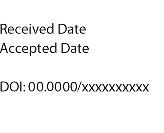
\includegraphics{head_foot/dates} & \\

\end{tabular}

 \end{@twocolumnfalse} \vspace{0.6cm}

  ]
%%%END OF TITLE AND AUTHORS%%%

%%%FONT SETUP - please do not change any commands within this section
\renewcommand*\rmdefault{bch}\normalfont\upshape
\rmfamily
\section*{}
\vspace{-1cm}


%%%FOOTNOTES%%%

\footnotetext{\textit{$^{a}$~PostEra Inc, 2 Embarcadero Centre, San Franciso, CA 94111, United States of America}}
\footnotetext{\textit{$^{b}$~Department of Physics, University of Cambridge, CB3 0HE, United Kingdom }}
\footnotetext{\textit{$^{c}$~The COVID Moonshot Consortium, \url{www.postera.ai/covid} }}
\footnotetext{\textit{$^{d}$~The Pritzker School for Molecular Engineering, The University of Chicago, Chicago, IL, USA }}
\footnotetext{\textit{$^{e}$~Computational and Systems Biology Program Sloan Kettering Institute, Memorial Sloan Kettering Cancer Center, New York, NY 10065, USA }}
\footnotetext{\textit{$^{f}$~Department of Organic Chemistry, The Weizmann Institute of Science, 76100, Rehovot, Israel }}

%Please use \dag to cite the ESI in the main text of the article.
%If you article does not have ESI please remove the the \dag symbol from the title and the footnotetext below.
\footnotetext{\dag~Electronic Supplementary Information (ESI) contains experimental and assay details. Our training set, de novo design method and generated molecules are available on \url{https://github.com/wjm41/mpro-rank-gen}.}
%additional addresses can be cited as above using the lower-case letters, c, d, e... If all authors are from the same address, no letter is required

\footnotetext{\ddag~These authors contributed equally to this work. }
\footnotetext{\P E-mail: alpha.lee@postera.ai }

%%%END OF FOOTNOTES%%%

%%%ABSTRACT%%%%

\sffamily{\textbf{The SARS-CoV-2 main viral protease ($\mathrm{M}^\mathrm{pro}$) is an attractive target for antivirals given its distinctiveness from host proteases, essentiality in the viral life cycle and conservation across coronaviridae. We launched the COVID Moonshot initiative to rapidly develop patent-free antivirals with open science and open data. Here we report the use of machine learning for \emph{de novo} design, coupled with synthesis route prediction, in our campaign. We discover novel chemical scaffolds active in biochemical and live virus assays, synthesized with model generated routes. }}\\

%The abstrast goes here instead of the text "The abstract should be..."

%%%END OF ABSTRACT%%%%

\rmfamily %Please do not remove this line.

%%%MAIN TEXT%%%%

%Intro to COVID19 and Moonshot

Coronaviruses are a family of pathogens that is frequently associated with serious and highly infectious human diseases, from the common cold to the SARS-CoV pandemic (2003, 774 deaths, 11\% fatality rate), MERS-CoV pandemic (2012, 858 deaths, 34\% fatality rate) and most recently the COVID-19 pandemic (ongoing pandemic, 1.7 million deaths up to Dec 2020). %However, to date there is no approved oral antiviral for coronavirus. 

The main protease ($\mathrm{M}^\mathrm{pro}$) is one of the best characterized drug targets for direct-acting antivirals \cite{pillaiyar2016overview,cannalire2020targeting}. $\mathrm{M}^\mathrm{pro}$ is essential for viral replication and its binding site is distinct from known human proteases, thus inhibitors are unlikely to be toxic \cite{jin2020structure,liu2020development}. Moreover, the high degree of conservation across different coronaviruses renders $\mathrm{M}^\mathrm{pro}$ targeting a fruitful avenue towards pan-cornavirus antivirals \cite{ullrich2020sars}. To date, most reported $\mathrm{M}^\mathrm{pro}$ inhibitors are peptidomimetics, covalent, or both \cite{cannalire2020targeting}. Peptidomimetics are challenging to develop into oral therapeutics, and covalent inhibitors incur additional idiosyncratic toxicity risks. We launched the COVID Moonshot consortium in March 2020, aiming to find oral antivirals against COVID-19 in an open-science, patent-free manner \cite{chodera2020crowdsourcing}. 

Here we report the prospective use of a simple model to rapidly expand hits. Starting from 42 compounds with $\mathrm{IC}_{50}$ within assay dynamic range ($<100 \mu$M) and 515 inactives, our model designed 5 new compounds predicted to have higher activity, together with predicted synthetic routes. All designs were were chemically synthesized and experimentally tested, and 3 have measurable activity against $\mathrm{M}^\mathrm{pro}$. The top compound has comparable $\mathrm{M}^\mathrm{pro}$ inhibition to the best in the training set, but with a different scaffold, and is active against the OC43 coronavirus in a live virus assay. 

%Describe GenChem 
Algorithmic \emph{de novo} design aims to automatically generate compounds that are chemically diverse, synthetically accessible and biologically active \cite{schneider2016novo}. Classic approaches apply heuristics to fragment and modify known active compounds, with the region of chemical space explored and synthetic accessibility constrained by those rules \cite{brown2004graph,patel2009knowledge,hartenfeller2012dogs}. Recent machine learning approaches explore chemical space in more abstract molecular representation space \cite{gomez2018automatic,segler2018generating}, but this often comes at the expense of synthetic accessibility \cite{gao2020synthesizability}. Our approach builds on rule-based fragmentation and molecule generation, but employs a method that combines regression and classification amid noisy data, and use of machine learning to predict synthesis routes. Our model comprises two parts: compound prioritisation and chemical space exploration. 

%describe ranking model + result 
Our compound prioritisation model aims to predict whether a designed compound is likely to be an improvement in activity over the incumbent. However, as is typical in the hit-expansion stage, bioactivity modelling is hindered by insufficient data where the majority of compounds are inactive, and noisy data as measurement variability increases for lower affinity compounds. Thresholding the data and framing the problem as classification of active/inactive would not allow us to rank compounds based on predicted improvement over the incumbent, yet the amount of measured bioactivity data and the measurement noise  makes a regression approach challenging.


To overcome both challenges, we develop a learning-to-rank framework \cite{duffy2010molecular,agarwal2010ranking}. Rather than training a regression model to predict the $\mathrm{IC}_{50}$ of a compound, we instead train a classifier to predict whether a compound is more or less active than another compound, with the input to the model being the \emph{difference} in molecular descriptors between the molecules (see Figure \ref{fig:roc_plot} for a schematic). This model accounts for both compounds with $\mathrm{IC}_{50}$ measurements and compounds that are simply inactive -- active compounds are ranked by their $\mathrm{IC}_{50}$, all inactives with no measurable $\mathrm{IC}_{50}$ are considered less active than active compounds, and inactive-inactive pairs are ignored. Further, we account for noise by only considering $\mathrm{IC}_{50}$ differences amongst actives above 5 $\mu M$. We use the FastAI Tabular model \cite{howard2018fastai}, with input features generated from concatenated Morgan, Atom Pair, and Topological Torsion fingerprints implemented in RDkit \cite{rdkit}, and dataset was randomly split into training (80\%) and testing (20\%); details about model implementation can be found in ESI and source code.


Figure \ref{fig:roc_plot} shows that our binary ranking model achieves an AUC of 0.88 (95\% CI: [0.83,0.96]) in ranking ligands within the test set, and AUC for 0.94 (95\% CI: [0.91,0.98]) where we compare a ligand in the training set against another ligand in the test set; the latter is more relevant as our goal is finding ligands more active than the best incumbent. The 95\% confidence interval is computed using bootstrapping. We also compare our model against OpenEye’s FRED hybrid docking mode as implemented in the ``Classic OEDocking'' floe, a physics-based docking algorithm, on the Orion online platform, which achieves AUC of 0.72; 95\% CI: [0.722,0.723] (see ESI for implementation details). Note that docking does not require ligand bioactivity as training data, thus is not a directly comparison to machine learning. In the Supplementary Material, we discuss that our model ranks ligands better than a model that directly learns $\mathrm{IC}_{50}$ (AUC = 0.86; 95\% CI: [0.71,0.95]). 

Beyond train-test split, model performance can be evaluated from a time-split. Five months have elapsed from the time we deployed our model to select compounds to writing up the manuscript. During that time, the COVID Moonshot Consortium (a team of expert medicinal chemists) has independently designed, synthesised and tested 356 compounds \cite{moonshot2020covid}, out of which 15\% were better than the top 2 compounds (having $\mathrm{IC}_{50}$ comparable within error) in our dataset. Table \ref{table:time_split} shows that our model has an enrichment factor of $\sim$2, i.e. if we rescore the 356 compounds synthesized by the medicinal chemistry team using our model, and pick the top 1\%-10\% percentile, the proportion of molecules that would be better than the top 2 compounds would be $\sim$2x higher than human selection. 

%From a set of binary ranking, we can accurately rank-order the active ligands (Figure XXXb), with a higher rank correlation than using the quantitative activity data alone. We use the average probability of a ligand being ranked higher than ligands in the training set as a proxy for overall rank.

\begin{figure}
\centering
    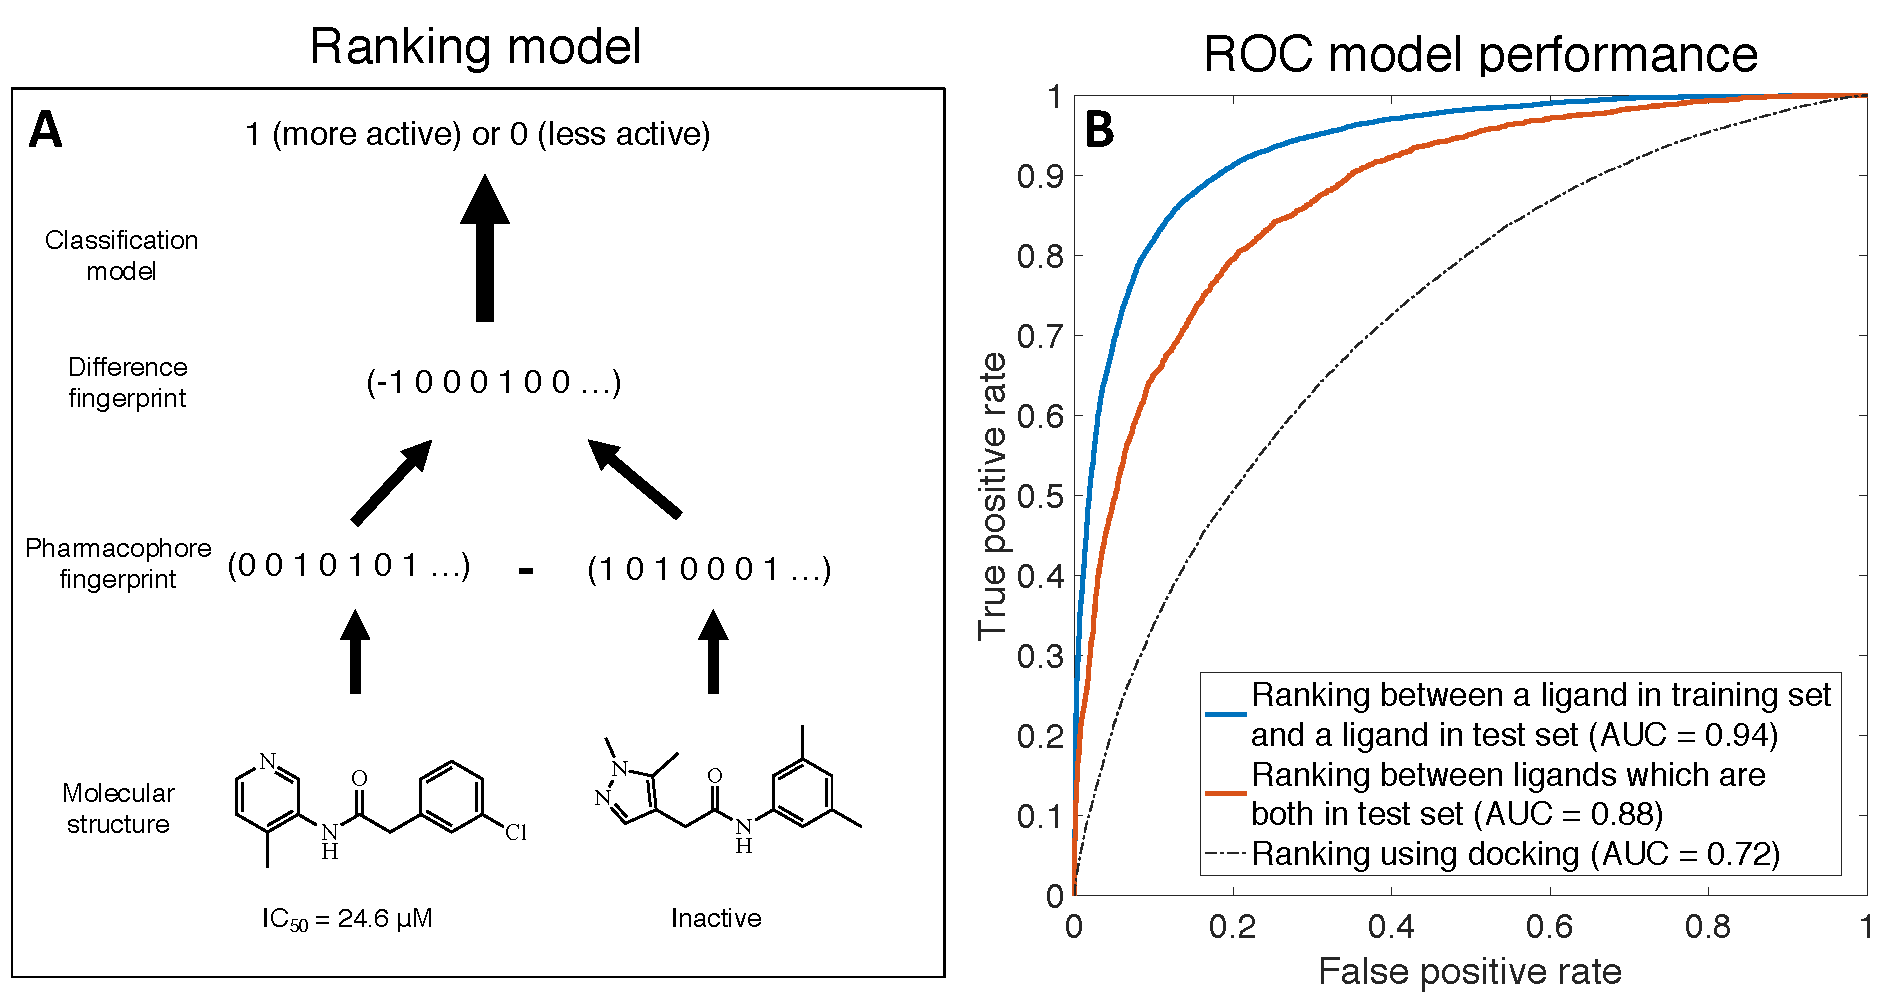
\includegraphics[scale=0.28]{ranking-model.pdf}
    \caption{Relative ranking of ligands can be predicted by our learning-to-rank machine learning model. (A) A schematic of the model setup. A classifier takes the difference in pharmacophore fingerprint between two molecules and predicts where one molecule is more or less active than the other. (B) The Receiver Operating Characteristic curve of classifying whether a molecule is more/less active than the other. AUC 95\% CI reported in main text.}
    \label{fig:roc_plot}
\end{figure}

\begin{table}
\centering
\begin{tabular}{|l|l|l|l|}
\hline
\textbf{Percentile}        & 1\% & 2.5\% & 10\% \\ \hline
\textbf{Enrichment Factor} & 1.7 & 2.3   & 1.7  \\ \hline
\end{tabular}
\caption{Enrichment factor for the time-split dataset, where we consider model performance on data arriving after the model has been deployed to generate compounds for synthesis and testing. }
\label{table:time_split}
\end{table}

\begin{figure}
\centering
         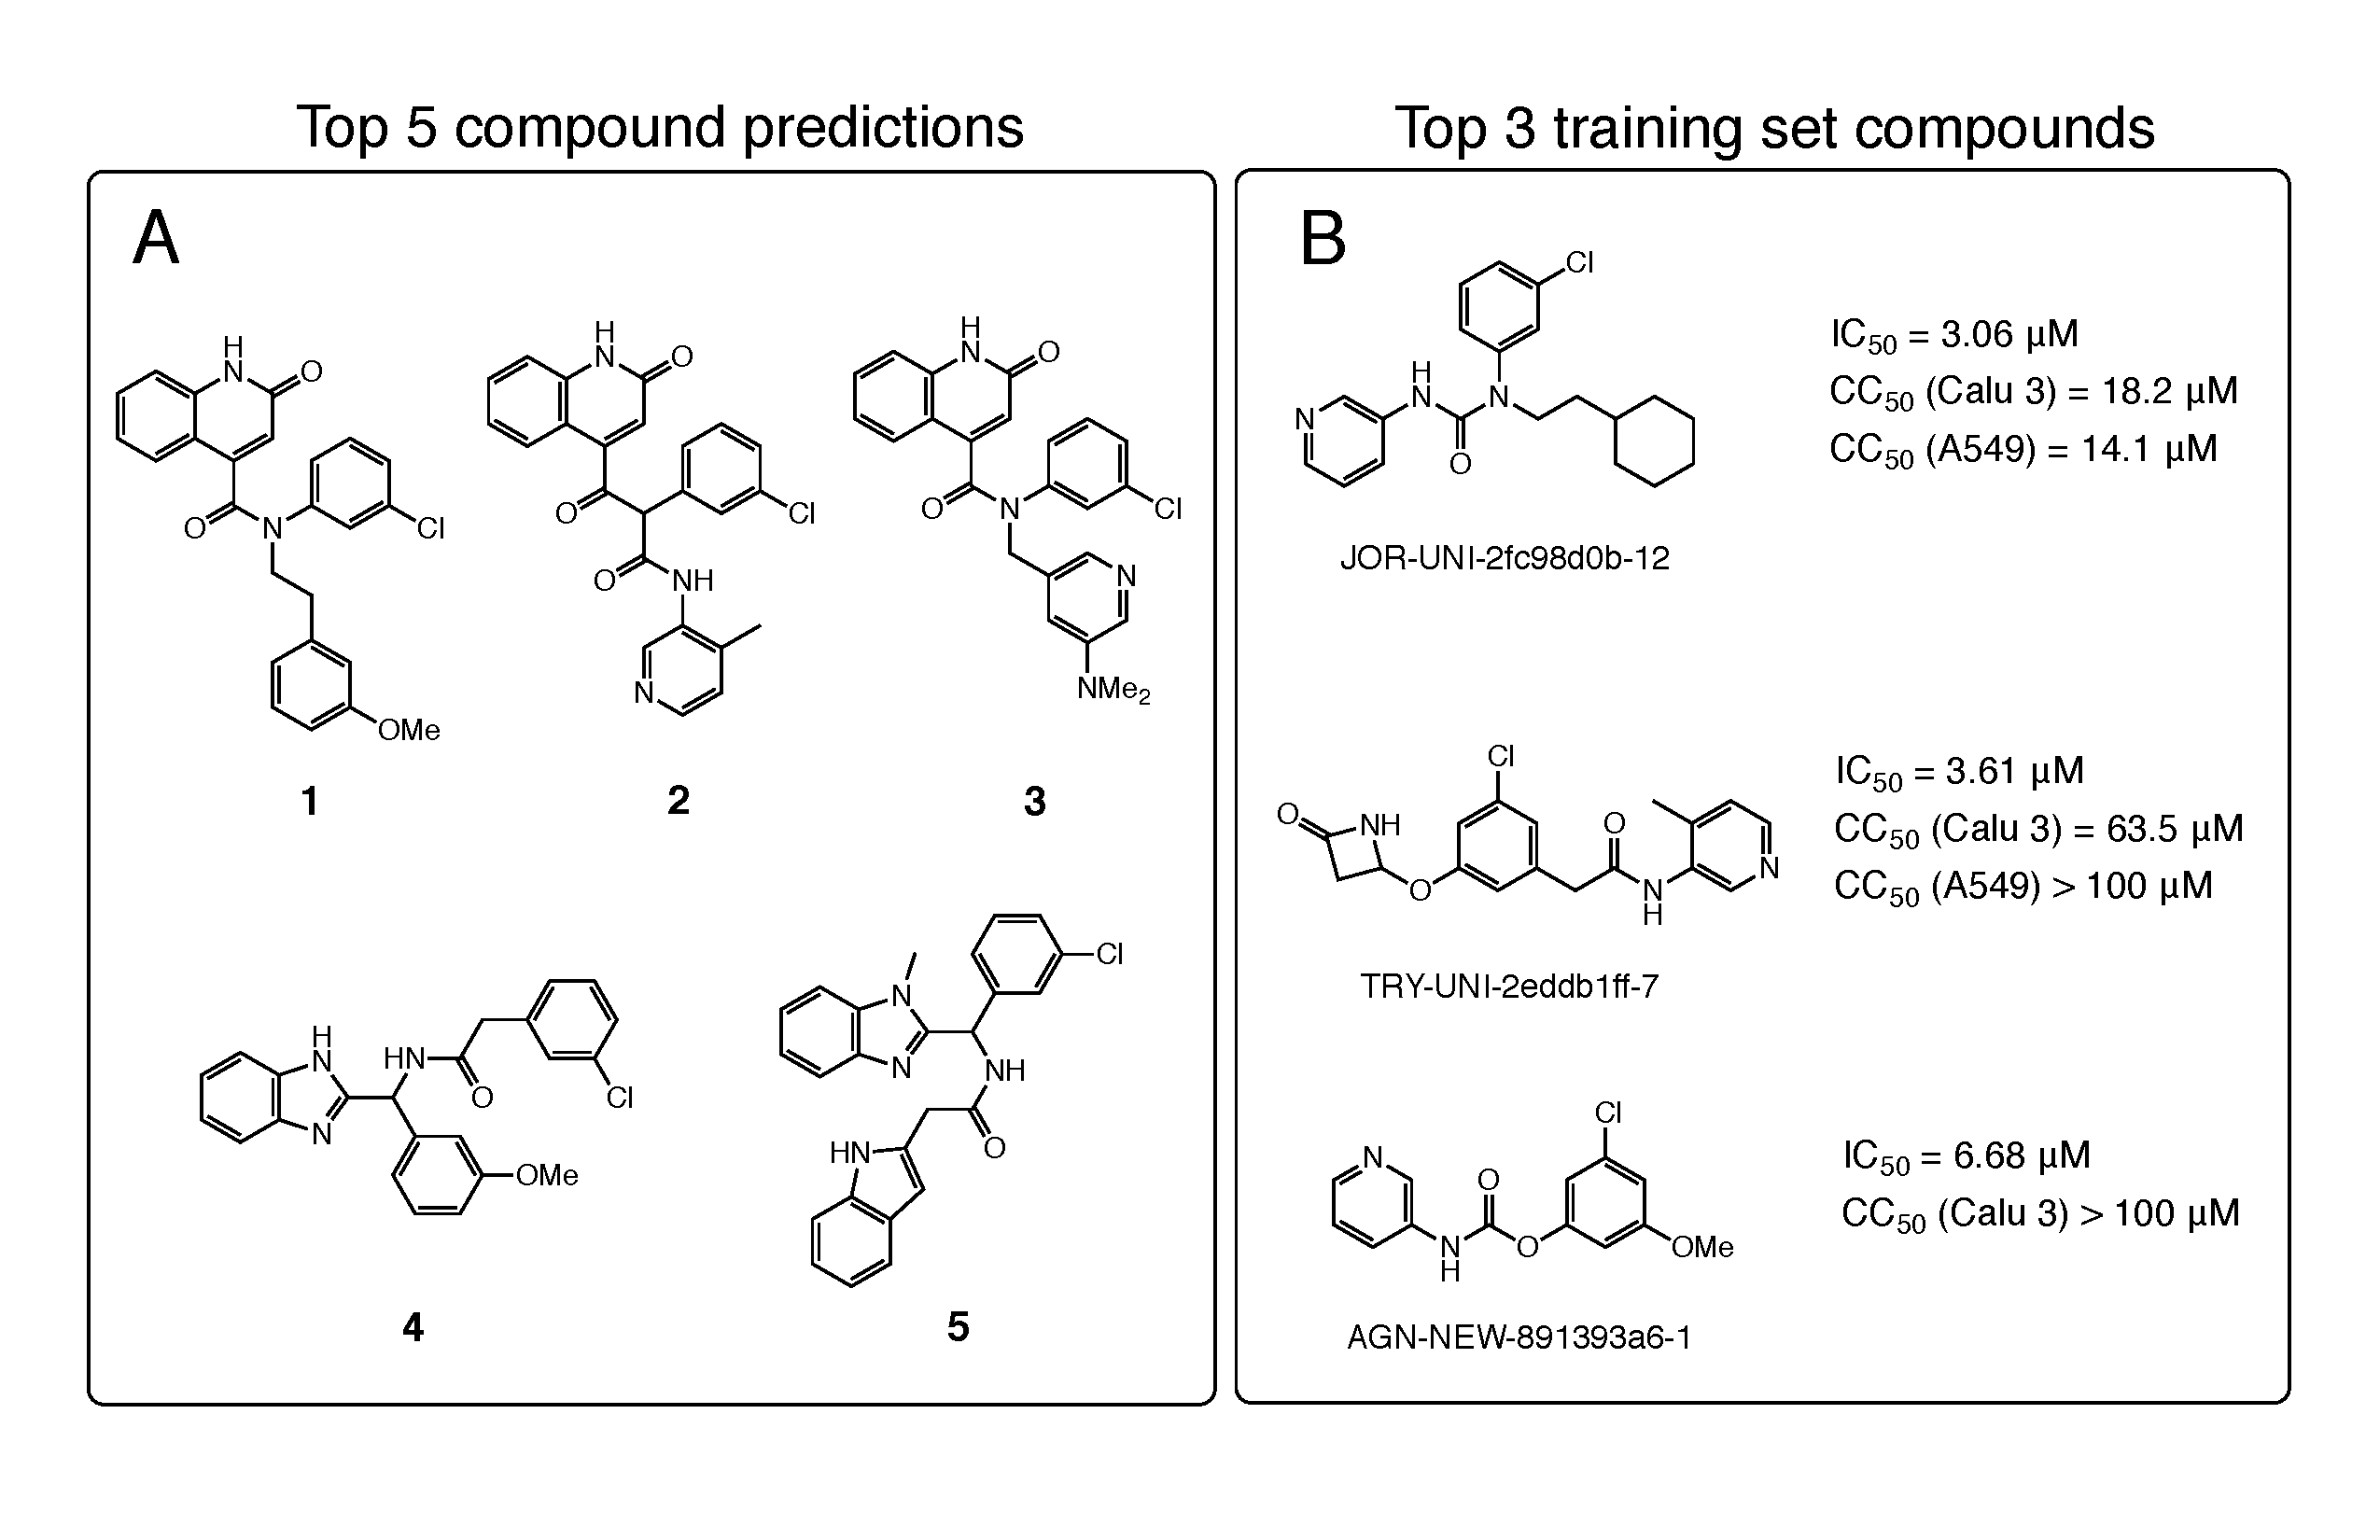
\includegraphics[width=0.45\textwidth]{fig2.pdf}
    \caption{Our synthesis-driven design model prioritises molecular scaffold that are not in the top hits. (A) The 5 compounds selected by our methodology for synthesis and testing. (B) The top 3 compounds from the training set, with potency and cytotoxicity measurements. }
    \label{fig:compounds}
\end{figure}


%describe our generative model + schematic 

Having demonstrated the accuracy of our ranking model, we now turn to chemical space exploration. We first consider a set of chemically reasonable perturbations (e.g. amide to retroamide, amide to urea), which is applied to the whole set of active molecules. We then fragment along synthetically accessible bonds (e.g. amides and aromatic C-C and C-N), and reconnect the synthons to generate an exhaustive library. The resulting library of 8.8 million generated molecules is scored using our ranking model by the probability of having a higher potency compared to the most potent molecule in the dataset.  % We use a simple scheme based on breaking along synthetically accessible bonds. 


\begin{figure}
\centering
         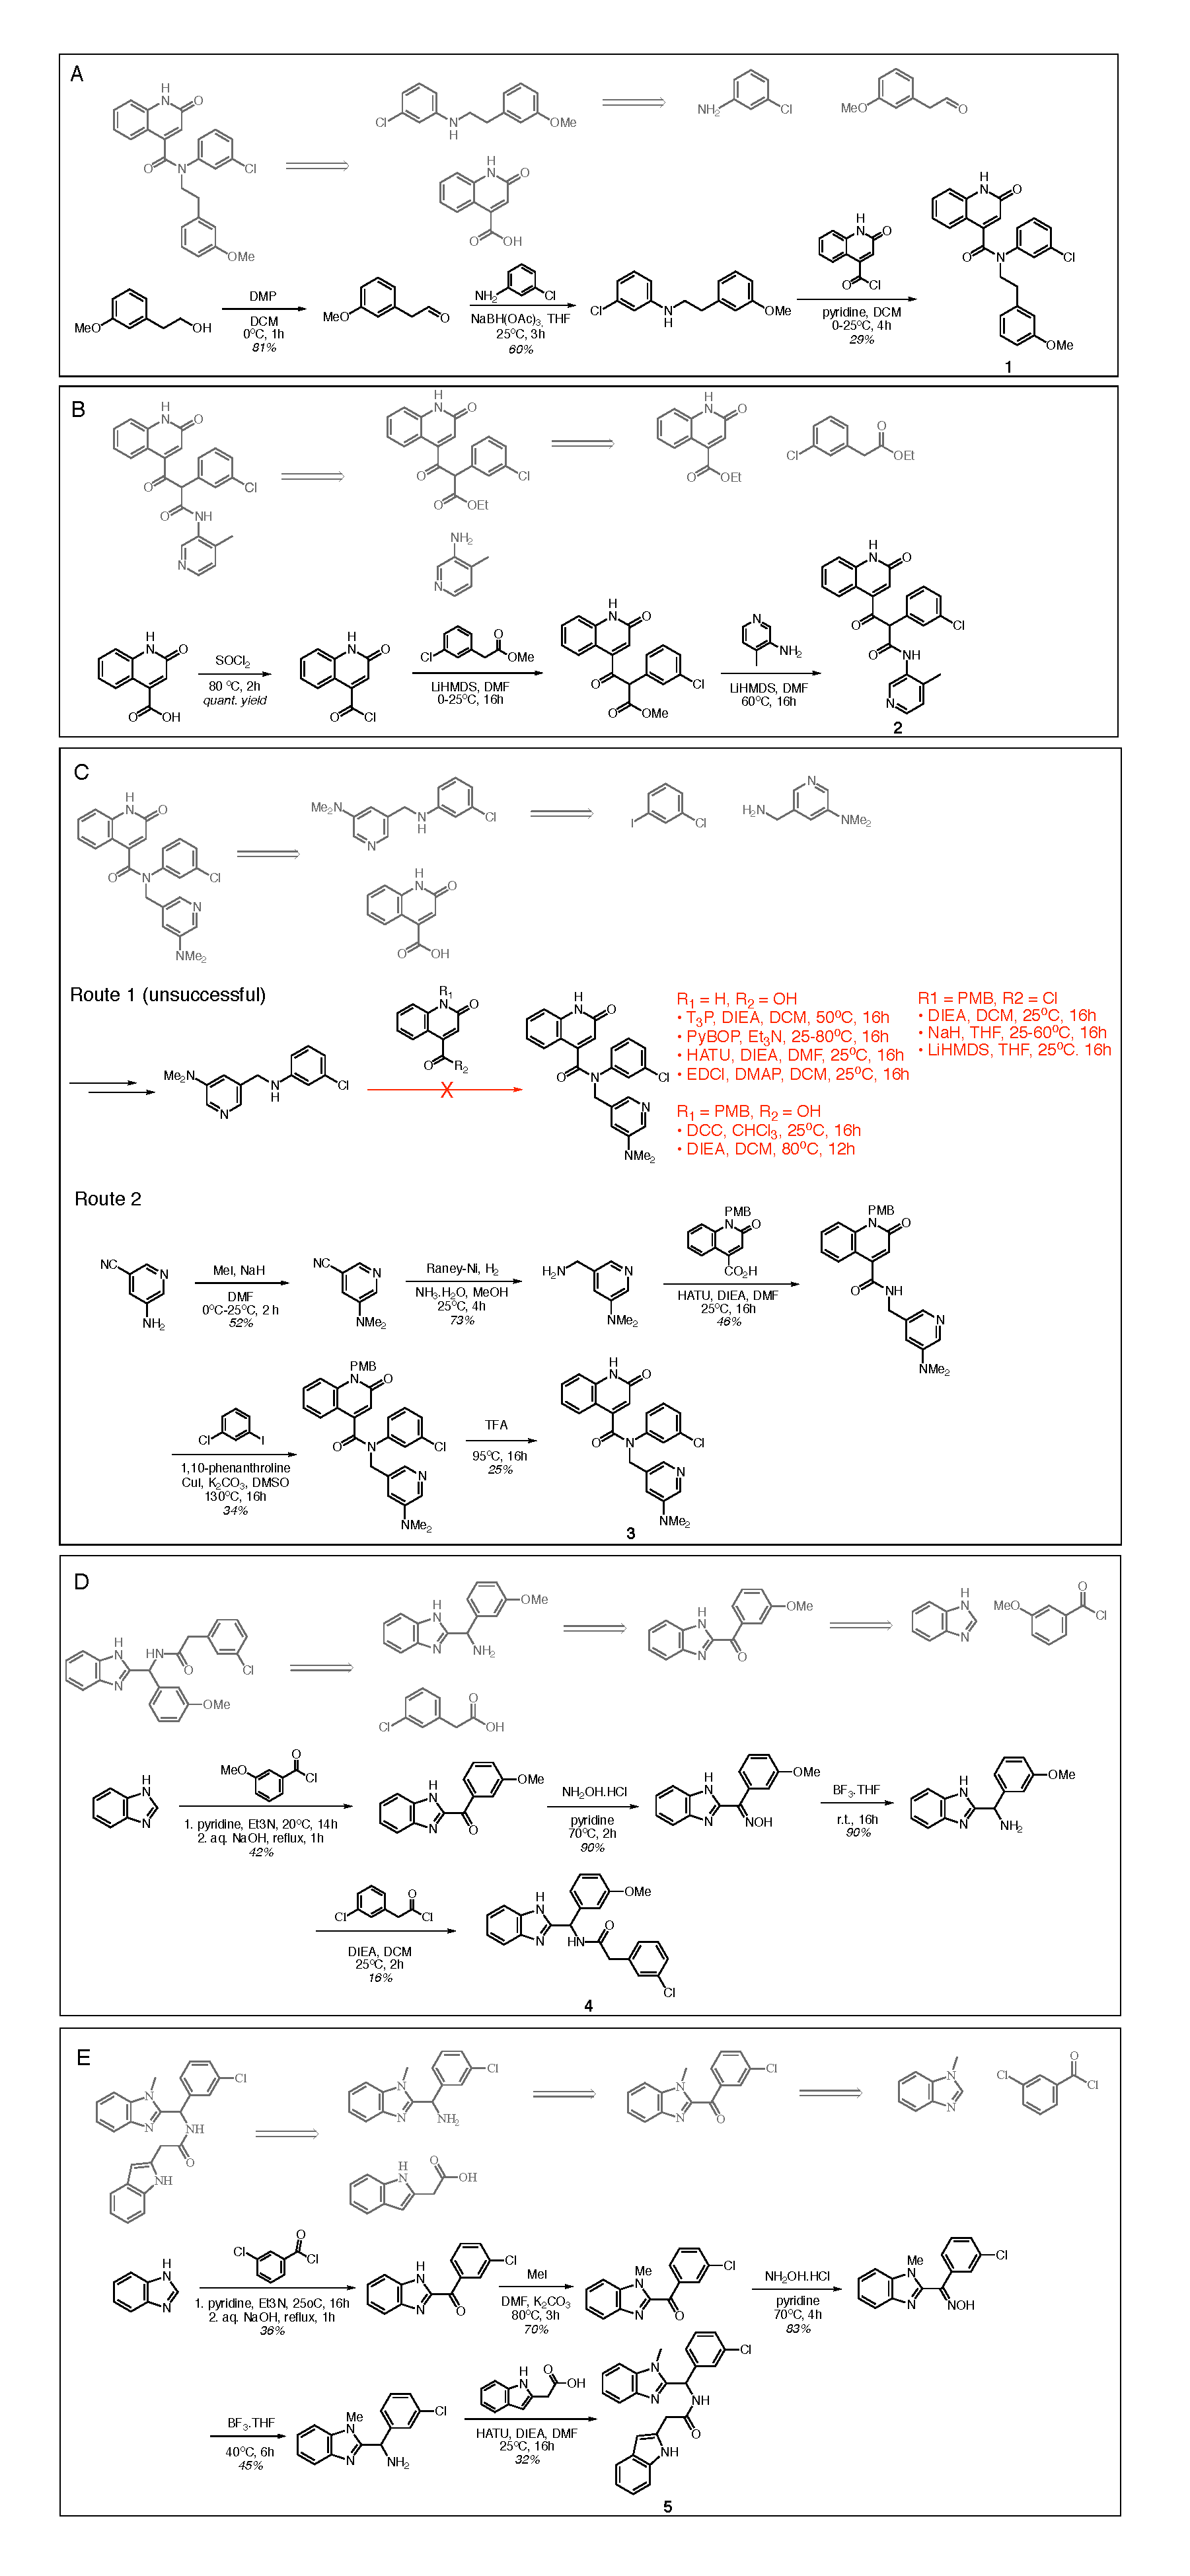
\includegraphics[width=0.5\textwidth]{aaron_schemes.pdf}
    \caption{Model generated synthetic schemes that are experimentally validated. Schemes (A)-(E) show the synthesis schemes generated by our model (grey) and experimental schemes for Compounds $\mathbf{1}$-$\mathbf{5}$. The ESI contains experimental procedures provided by our contract research organisation.}
    \label{fig:synthesis_schemes}
\end{figure}

Although virtual ``reactions'' were used to generate new molecules, the synthons are not necessarily off-the-shelf nor the reactions optimal. As such, we use a retrosynthesis predictor to triage based on synthetic accessibility. We fed top hits into Manifold, our platform for synthesis route prediction (\url{https://postera.ai/manifold}). Manifold searches for synthetic routes starting from purchasable molecules. The underlying technology is based on Molecular Transformer, a machine learning model for reaction prediction using sequence-to-sequence translation \cite{yang2019molecular,schwaller2019molecular}. The top 5 molecules with predicted routes <4 steps were synthesised and tested (Figure \ref{fig:compounds}A). For comparison, the most potent molecules from the training set are shown in Figure \ref{fig:compounds}B; $\mathbf{1}-\mathbf{5}$ have Tanimoto similarity <0.48 (1024-bit ECFP6) to every molecule in the training set. 


Figure \ref{fig:synthesis_schemes} shows that for Compounds $\mathbf{1}$, $\mathbf{2}$, $\mathbf{4}$ and $\mathbf{5}$ our retrosynthesis algorithm generates successful routes, thus provides a reasonable estimate of synthetic complexity. The syntheses were carried out at the Wuxi AppTec and compounds were assayed as received. Minor variations in building blocks were employed depending on what was readily available. We note that our algorithm failed to estimate the synthetic complexity of Compound $\mathbf{3}$. The final amide formation step was unexpectedly challenging, and no desired product was seen despite significant efforts in condition screening. Compound $\mathbf{3}$ was furnished via an alternative strategy, employing an Ullmann coupling to arylate the amide, which was not predicted by our approach. 

%result + discussion 
Compounds $\mathbf{1}$-$\mathbf{5}$ were tested for Mpro activity using a fluorescence assay. Figure \ref{fig:data} shows that Compounds $\mathbf{1}$-$\mathbf{3}$ have $\mathrm{IC}_{50}$ within assay dynamic range ($<100 \mu M$), and Compound $\mathbf{1}$ has $\mathrm{IC}_{50} = 4.1 \mu M$. Compound $\mathbf{1}$ is further assayed in live virus assays, with the less pathogenic OC43 coronavirus, showing $\mathrm{EC}_{50} = 13 \mu M$ and is not cytotoxic ($\mathrm{CC}_{50}>100 \mu M$ against A549 cell line; $CC_{50}$ is the concentration required  to cause 50\% cell death). We employ OC43 as a rapid surrogate assay for SARS-CoV-2 as the former can be done in a BSL-2 rather than BSL-3 lab.  Interestingly, the top non-cytotoxic hit of the training set (TRY-UNI-2eddb1ff-7) does not show OC43 activity, showcasing the utility of using generative models to suggest new scaffolds with complementary physicochemical properties. 

\begin{figure}
\centering
         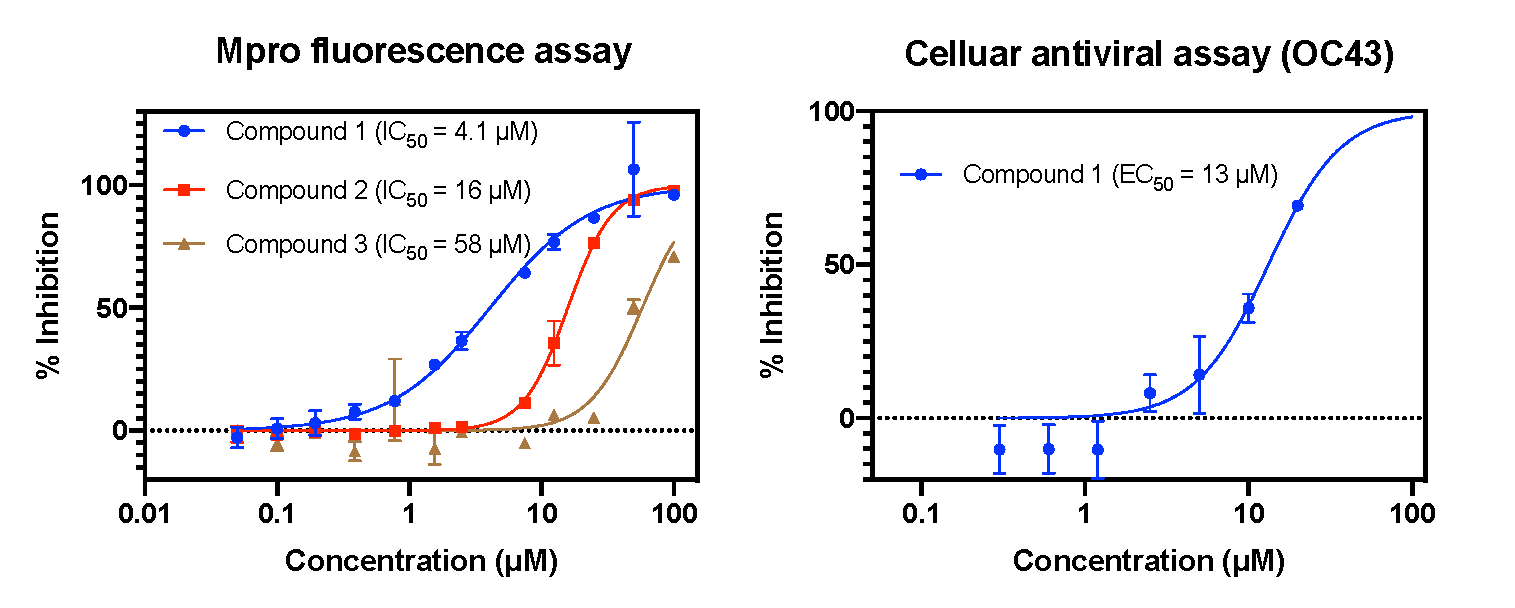
\includegraphics[scale=0.36]{data_curve.pdf}
    \caption{Three compounds generated using our synthesis-directed model exhibit Mpro activity. Our most active compound has measurable antiviral activity against the OC43 coronavirus and no measurable cytotoxic effect ($\mathrm{CC}_{50} (A549)>100 \mu M$). 95\% CI: IC50 (Mpro) -- Compound 1 [3.42,4.86] $\mu$M, Compound 2 [15.1,16.5] $\mu$M, Compound 3 [48.8,69.4] $\mu$M; EC50 (OC43) -- Compound 1 [10.1, 18.4] $\mu$M. See ESI for assay details.}
    \label{fig:data}
\end{figure}

In summary, we demonstrated the utility of a \emph{de novo} design model, guided by estimation of synthetic complexity, for generating ideas in hit expansion. At the time of writing, the quinolone series is undergoing optimisation by the COVID Moonshot initiative (\url{https://postera.ai/covid}). Data for Compound $\mathbf{1}$-$\mathbf{5}$ is registered as the $\texttt{ALP-POS-ddb41b15}$ series on the Moonshot platform. 

%You can also put lists into the text. You can have bulleted or numbered lists of almost any kind. 
%The \texttt{mhchem} package can also be used so that formulae are easy to input: \texttt{\textbackslash ce\{H2SO4\}} gives \ce{H2SO4}. 


%The conclusions section should come at the end of article. For the reference section, the style file \texttt{rsc.bst} can be used to generate the correct reference style.\footnote[4]{Footnotes should appear here. These might include comments relevant to but not central to the matter under discussion, limited experimental and spectral data, and crystallographic data.}

\section*{Acknowledgements}
JDC acknowledges support from NIH grants P30 CA008748 and GM124270. 

\section*{Conflicts of interest}
A.M. and A.A.L are co-founders and shareholders of PostEra (\url{https://postera.ai}). J.D.C is a current member of the Scientific Advisory Board of OpenEye Scientific Software, Interline Therapeutics, and Redesign Science. The Chodera laboratory receives or has received funding from multiple sources,including the National Institutes of Health, the National Science Foundation, the Parker Institute for Cancer Immunotherapy, Relay Therapeutics, Entasis Therapeutics, Silicon Therapeutics, Interline Therapeutics, EMD Serono (Merck KGaA), AstraZeneca, Vir Biotechnology, Bayer, XtalPi, the Molecular Sciences Software Institute, the Starr Cancer Consortium, the Open Force Field Consortium, Cycle for Survival, a Louis V. Gerstner Young Investigator Award, and the Sloan Kettering Institute. A complete funding history for the Chodera lab can be found at \url{http://choderalab.org/funding}.
%%%END OF MAIN TEXT%%%

%  For footnotes in the main text of the article please number the footnotes to avoid duplicate symbols. e.g.  \footnote[num]{your text} the corresponding author \ast counts as footnote 1, ESI as footnote 2, e.g. if there is no ESI, please start at [num]=[2], if ESI is cited in the title please start at [num]=[3] etc. Please also cite the ESI within the main body of the text using \dag.

% The \balance command can be used to balance the columns on the final page if desired. It should be placed anywhere within the first column of the last page.

% \balance

% If notes are included in your references you can change the title from 'References' to 'Notes and references' using the following command:
% \renewcommand\refname{Notes and references}

%%%REFERENCES%%%
\scriptsize{
\bibliography{rsc} %You need to replace "rsc" on this line with the name of your .bib file
\bibliographystyle{rsc} } %the RSC's .bst file

\end{document}

%!TEX root = ../thesis.tex
%*******************************************************************************
%****************************** Second Chapter *********************************
%*******************************************************************************

\chapter{Make - Understanding the Molecular Transformer}
\label{chap:MolTrans}
\section{Introduction}
\label{sec:int}
Although the design of drug candidates is exhaustingly difficult, it is in fact the `make' part of the design-make-test cycle which is the most costly, time consuming and labour intensive. The key to streamlining molecular synthesis is in improving route planning, developing faster ways of designing shorter reaction paths from basic molecular building blocks to the desired molecule, reducing the number of steps and hence the risk of failure.

Once a synthesis route is designed it is important to validate each step of the plan. Forward chemical reaction prediction is concerned with predicting the (major) product of an organic reaction given the reactants, reagents and preferably the conditions like solvent, temperature, concentrations etc. By having the ability to predict the product of reactions with reliable uncertainties it is possible to design clever synthesis plans where the reactions with higher uncertainty are put first. This way if a synthesis protocol fails it does so fast and cheap instead of in the later stages of the route where substantial time and cost would go to waste.

Route planning and reaction prediction have traditionally been done by expert chemists relying on experience, as well as reaction databases like Reaxys \cite{ElsevierReaxysDatabase}. Nowadays, Computer Assisted Synthesis Planning tools are increasingly being used \cite{Coley2018}, as these tools can memorise libraries of commercially available building blocks and quickly evaluate large numbers of possible bond disconnections via efficient algorithms such as Monte Carlo Tree Search \cite{Segler2018PlanningAIb}. Unsurprisingly, machine learning methods have also entered into the fray \cite{Coley2019AutonomousOutlook, Coley2019AutonomousProgress} and have recently emerged as the most successful approach \cite{Coley2018, Schwaller2019MolecularPrediction}.

ML reaction prediction models are trained on reaction data that is extracted from patents and publications. In these documents usually the metadata about reactions like the temperature, concentrations and solvents are found in the synthesis protocol section making it very challenging to extract this information in an automated manner. Therefore these models are usually trained only on the reactants and reagents with all of the context information missing. In spite of this there are reported models achieving remarkably high near 90\% Top-1 prediction accuracy on these datasets, even outperforming quantum mechanics-based approaches \cite{Schwaller2019MolecularPrediction}. 

The natural question that arises is: how is the model able to achieve such high accuracy on often rather challenging reactions from such limited source of data? Has the model learnt the well-established underlying mechanistic drivers of reactivity purely from data? It is of utmost importance to validate these models to see if they are able to generalize and predict the outcome of reactions reliably or if they are merely learning hidden biases in the datasets which results in the seemingly strong performance. 

One way to accomplish this is with ML interpretability methods \cite{Alvarez-Melis2018OnMethods}. Interpretability methods can help uncover the reasoning of model predictions in simple well understood cases where the physical or chemical cause for certain outcomes is well established. For chemical reaction prediction our understanding of mechanisms and selectivities serves as good guides for the observed reactivities.

In this work, we use a well-known ML interpretation method called Integrated Gradients (IGs) to probe the understanding of the Molecular Transformer (MT), the current state-of-the-art machine learning model for chemical reaction prediction. Our approach builds on the work of McCloskey et.\,al.\,\cite{McCloskey2019UsingChemistry} who used IGs to understand binding prediction models on artificial datasets. We extend the method to Transformer architectures, and use it in the context of reaction predictions on real experimental data. We also present a novel method for attributing the predictions of neural network models to training set datapoints. With these tools we show that MT often fails to learn the mechanistic reasoning behind chemical selectivity and hypothesize that this is due to hidden biases in the dataset. We justify this claim by creating biased synthetic datasets and demonstrating selectivity bias in the model predictions, suggesting that it is the quality of training data rather than the particulars of model architectures that is constraining the potential for ML reaction prediction.

The work in this chapter was done collaboratively with D\'{a}vid P\'{e}ter Kov\'{a}cs. We did the code development together and discussed all of the results of the work. He executed the code, analysed the model attributions, and designed the majority of the experiments and all of the adversarial examples. I created the SMARTS templates for counting statistics from the patent datasets as well as for dataset generation in the synthetic experiments. Preliminary results from this work were presented at the ICML 2020 `ML Interpretability for Scientific Discovery' Workshop \cite{Kovacs20unpack}. All code including a \texttt{README} with the usage can be found in the GitHub repo \texttt{MTExplainer} \cite{Kovacs2020MolecularExplainer}.

\section{Methods}

\subsection{Molecular Transformer}
The Molecular Transformer \cite{Schwaller2019MolecularPrediction} is a tailored version of the Transformer architecture \cite{Vaswani2017} which was designed for machine translation and has had wide-ranging success in many Natural Language Processing tasks. It has an encoder-decoder structure, where both the encoder and the decoder are made up of so called transformer blocks. These blocks process the inputs by applying a multi-head scaled dot-product attention mechanism followed by layer normalization and some fully connected feed forward layers. Mathematical details can be found in (somewhere).

The string input to the model is broken down into individual tokens with a learnt embedding that is fed into the encoder layer with positional encoding. The encoder is composed of 4 identical attention blocks each containing a multi-head self-attention layer and a 2-layer fully connected feed-forward neural network. The decoder is very similar to the encoder with the only difference being that the multi-head attention uses the output of the encoder as the keys and the values with the output of the previous decoder layer being the query. The predictions are generated in an autoregressive way meaning that the decoder predicts one token at a time and the previously generated tokens are fed into the decoder when generating the next tokens. The prediction is considered final when an \texttt{<end>} token is generated or the maximum length is reached. Through this process each translation gets assigned a probability score:
\begin{equation}
    P(\textrm{tgt} \mid \textrm{src}) = \prod_{i=1}^N P(\textrm{tok}_i \mid \textrm{tok}_1, \cdots , \textrm{tok}{i-1}, \textrm{src}) 
\end{equation}
where $\textrm{tok}_i$ is the $i$-th predicted token and $N$ is the length of the prediction.

Our implementation of the work was based on the \texttt{OpenNMT} package \cite{Klein2017}.

\subsection{Data}
We trained the model on a publicly available dataset of organic reactions mined from the US patent office \cite{Lowe2012} which has been filtered \cite{Jin2017}. The data contains reactants, reagents, and products represented as SMILES (without including stereochemical information) which is a text based representation of molecules\cite{Weininger1988, Weininger1989}. The training set was made up of 377 419 reactions which we augmented by an equal number of identical reactions made up of random equivalent SMILES. This augmentation is done to help the model to learn the underlying molecular graph from the SMILES sequence.There were 23 589 reactions for the validation set and 70 765 reactions in the hold-out test set, neither of which were augmented. The SMILES strings were tokenized following \cite{Schwaller2019MolecularPrediction}.

The trained model achieved 88.8\% Top-1 accuracy on the test set. This model was used throughout the interpretability experiments and is referred to as USPTO Transformer.

The second dataset used was the commercial Pistachio dataset \cite{Mayfield2018Pistachio2.0}. This dataset contains over 9 million reactions text mined from US and EPO patents. This dataset was filtered similarly to USPTO to remove erroneous and and a large number of duplicate reactions. The final dataset consisted of 2 375 385 reactions, of which 2 019 078 were used for training, 118 770 for validation and 237 537 for testing. 

The model trained as described above achieved 76.4\% Top-1 accuracy on the test set. Even though this looks like a substantially lower performance in reality the two models perform similarly well on new reactions. The possible reasons for the large difference in the measured performance on the held-out test sets are described in detail below. This model obtained was also used in the interpretability experiments to test the effect of increased training set size on the models understanding of chemistry and is referred to as Pistachio Transformer from here onwards. 

\subsection{Integrated Gradients}
To understand the predictions of MT with respect to the input features, we use the Integrated Gradients \cite{Sundararajan2017AxiomaticNetworks} attribution method. Integrated Gradients (IGs) is a principled model-agnostic feature attribution method adapted from game theory which obeys certain axioms of fairness. It can be used for any model where gradients are available, which is the case for all neural networks that are trained by some variant of gradient based optimization.

In general, the attribution of feature $i$ for input $x$ is given by
\begin{equation}
\label{eqn:IG}
    IG_i(x) = (x_i - x_i') \int_{\alpha=0}^1 \frac{\partial F(x' + \alpha(x-x'))}{\partial x_i} d\alpha
\end{equation}
where $x_i$ is the vector of feature $i$ for the input $x$, and $x_i'$ is a vector corresponding to a non-informative baseline input, $F(x)$ represents the model prediction for input $x$, and the integral is taken over the straight-line path from the baseline to the input of interest. 

It has been discussed before that the choice of baseline can have a large effect on the values of the attributions \cite{sturmfels2020visualizing}. While we could have chosen unreactive molecules as our baseline, it is important to select baselines which are completely non-informative to avoid any ambiguity. This would traditionally be the black image in the case of image recognition. In this work we use the embedding vector of the SMILES ` \textbf{.} ' token which is used to separate different molecules and hence does not contain any chemical information on its own.

For MT, we take great care to define $F(x)$ as it is not an appropriate question to ask what part of the reactant-reagent input is most important for predicting a given product. All of the input tokens contain crucial information that are used by the decoder to generate the entire target structure correctly. To eliminate this effect we define $F(x)$ as the difference in predicted probability of two possible products. Since the inert parts of the input are the same for the two products they should not substantially contribute to their predicted probability difference. This method is especially suited for examining reactions with selectivities. In other words we attribute the selectivity between two products to the inputs, ideally highlighting the chemically important groups driving this selectivity (by summing the attributions of the tokens comprising these groups).

If it is found that the correct product is predicted for the wrong reason i.e. the attribution on the chemical important group is low, it can be confirmed that model has not been able to learn the underlying chemistry through the construction of adversarial examples. In these examples we only change the parts that are chemically important, but not according to the model. This way the model can be fooled into incorrect predictions if the interpretation is correct, or the interpretation can be falsified if the model is able to predict the correct product. This is a crucial element of our method as any interpretation that cannot be falsified would be no more than speculation.

When talking about the size of an attribution we always compare it to the amount of attribution the group would get if the probability difference would be distributed uniformly across the input tokens. This serves as a way of normalizing the attributions by the size of the different substructures. We consider the parts of the reactant that get substantially higher attribution than expected to be `important'.

\subsection{Data Attribution}
In cases when a model predicts something very unexpected to humans attributions to parts of the input can be difficult to make sense of. Sometimes it can be much more illustrative to attribute to data instead and see a couple of example inputs that the model finds similar, which can reveal biases that the model has learnt.

To successfully attribute to data, we must understand how `similar' two input datapoints are according to the model by defining a similarity metric. For the Molecular Transformer which has an encoder-decoder architecture we use the output of the encoder layers as a basis for comparing data points. The challenge lies in the fact that these encoder hidden states have a non-fixed length $256\times N$ where $N$ is the length of the input sequence. To overcome this we average these vectors over the sequence dimension $N$, obtaining a representation of fixed size 256. We hypothesized that averaging can work because of the relatively large dimensionality and hence sparsity of the embedding space, allowing the averaged vector to retain most of the information about the structure, reagents and reactivity. 

We generated these averaged encoder state vectors for all of the reactions in the training sets. When a new example input is given it is passed through the Transformer encoder and the average hidden state vector of it is calculated. The similarity score of this vector to the training set vectors is calculated by
\begin{equation}
    score = \frac{1}{1 + D}
\end{equation}
where $D$ is the Euclidean distance between the vectors. This can be implemented in a vectorized way resulting in very quick computation even in the case of dataset sizes like Pistachio made up of over 2 million training examples. The top-$n$ most similar reactions are returned where $n$ is defined by the user. A similar approach is used in \cite{Allen2020} to measure the model-learned similarity between molecules for a graph neural network trained on toxicity prediction. These similarities are also used as evidence for judging the reliability of the model predictions, but only for unseen molecules not in the training set. In this work we go beyond assessing reliability into explaining the failures of the model by explicitly examining the training data itself to reveal hidden biases.

% From each reaction type we design a representative reaction that contained some selectivity and produce predictions with the USPTO and Pistachio Transformer. In the case of correct predictions the IG attributions were generated and evaluated whether they agreed with the underlying chemical causes of selectivity or not. After that based on the IGs a number of adversarial examples were generated to either confirm that the model is making the right prediction for the right reason or to confirm that the interpretation is correct and the model did not learn the underlying chemical causes. Attributions to training data were also generated to help confirm that the model is correctly making predictions based on chemically similar examples and also to help identify the causes of incorrect predictions. The causes found include the absence of similar reactions in the training set, erroneous training datapoints and biases in the training set. 

\begin{figure}[htbp!] 
\centering    
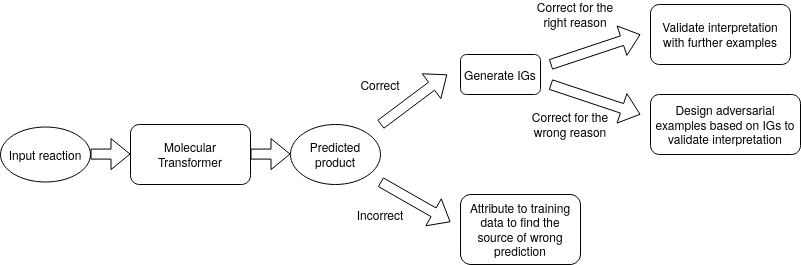
\includegraphics[width=1.05\textwidth]{Chapter4/Figs/workflow.png}
\caption[workflow]{An overview of the workflow for interpreting the Molecular Transformer.}
\label{fig:workflow}
\end{figure}

\section{Results}
To interpret the predictions of the Molecular Transformer we follow an analysis workflow (Fig~\ref{fig:workflow}) and examine a number of reaction types that are commonly used in synthetic organic chemistry using both input and data attribution techniques.
\subsection{Diels-Alder reactions}
The Diels-Alder reactions transform a conjugated diene and an alkene (called dienophile) to a six membered ring with a double bond \cite{Clayden2012}. A typical example is shown in Fig~\ref{fig:da1}. Diels-Alder reactions are regioselective meaning that the methoxy and nitrile group can be opposite or one carbon apart on the ring formed as shown in Fig~\ref{fig:da1}. The major product is the one marked TRUE on the figure because of more favourable HOMO-LUMO interactions. Due to the large number of possible products and complicated rules determining the major product the Diels-Alder reaction can serve as a challenging test for any reaction prediction model.

\begin{figure}[htbp!] 
\centering    

\includegraphics[width=0.9\textwidth]{Chapter4/Figs/da1.png}
\caption[Diels-Alder]{A typical example of a Diels-Alder reaction with challenging selectivity.}
\label{fig:da1}
\end{figure}

\begin{figure}[htbp!] 
\centering    
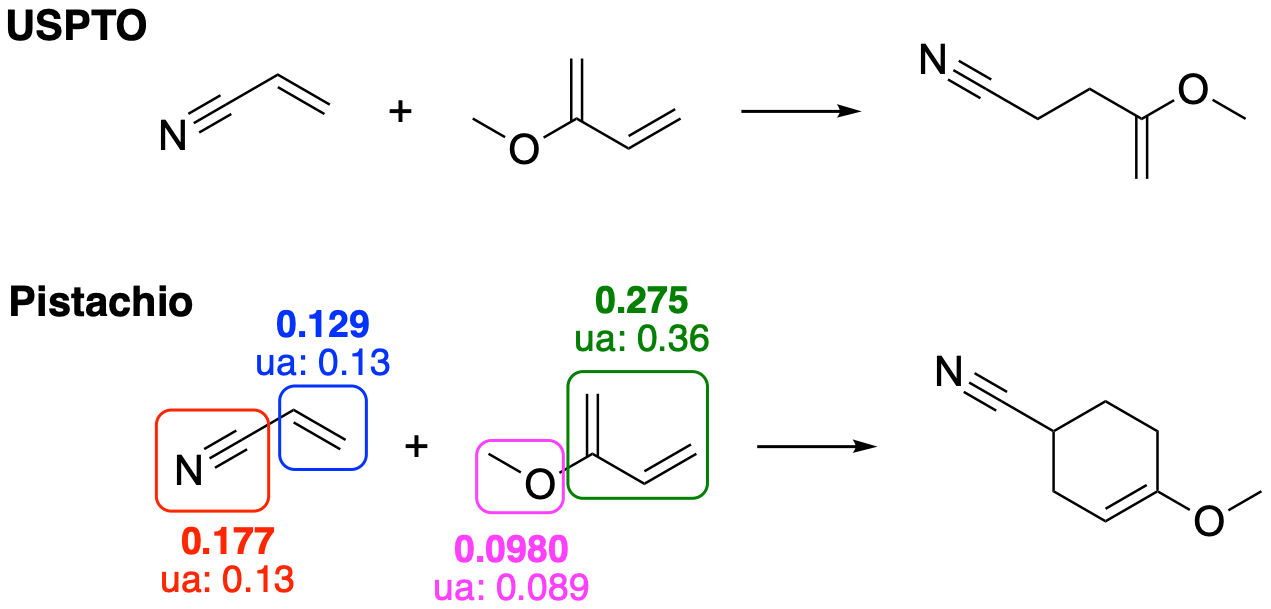
\includegraphics[width=0.8\textwidth]{Chapter4/Figs/da1_preds.png}
\caption[Diels-Alder]{The USPTO transformer makes a completely incorrect prediction, while the Pistachio model correctly predicts the product and recognises the importance of the nitrile group. For the Pistachio model the IG attributions are shown together with the corresponding uniform attribution (ua) values. }
\label{fig:da1_preds}
\end{figure}

Fig~\ref{fig:da1_preds} shows the Top-1 prediction of the USPTO and Pistachio models. The USPTO model does not seem to recognize the Diels-Alder reaction and gets the prediction wrong, indicating its own uncertainty by assigning a very low score of 0.300 to the prediction. To find the reason for the wrong prediction we attributed to training data (Fig~\ref{fig:da1_uspto_dat}). The first reaction seems to be an erroneous datapoint whereas the other two are different carbon-carbon bond formation reactions. This indicates that either the model has not learnt to recognize Diels-Alder reactions or the dataset did not contain any of them. 

\begin{figure}[htbp!] 
\centering    

\includegraphics[width=1.0\textwidth]{Chapter4/Figs/da1_uspto_dat.png}
\caption[Diels-Alder]{Attribution to the USPTO training data shows that the USPTO transformer either completely fails to recognize Diels-Alder reactions or that no Diels-Alder reactions exist in the dataset. }
\label{fig:da1_uspto_dat}
\end{figure}

To check this we devised a simple reaction template of Diels-Alder reactions and ran a template matching algorithm on the training data. We validated the template by ensuring it was able to identify the reactions where a diene and a double bond participate in cyclo-addition, which made up 80\% of the $\sim$2.3k labelled Diels-Alder reactions in Pistachio. This template matched only 7 reactions in the USPTO dataset confirming that it contains very few instances of this type of reaction. Furthermore this suggests that the model was not able to generalize across chemical space to infer this reactivity from different types of reactions. This level of generalization could only be expected from physics based models that have direct access to quantum mechanical information driving the reactions.

\begin{figure}[htbp!] 
\centering    

\includegraphics[width=1.0\textwidth]{Chapter4/Figs/da1_adv.png}
\caption[Diels-Alder]{Further test reactions correctly predicted by the Pistachio model, validate that Pistachio correctly understands Diels-Alder reactions. \cite{Husinec2011AnnulationsDerivatives, Tiamas2018AsymmetricChalcones}}
\label{fig:da1_adv}
\end{figure}

For the Pistachio model the Top-1 prediction is correct, as shown in Fig~\ref{fig:da1_preds}, and it has a confidence score of 0.819 indicating that it is fairly certain in the prediction. We also generated the IGs for this reaction to see if the selectivity is caused by the relevant nitrile and methoxy groups. The probability difference between the correct major and the minor products was 0.77 and it was distributed on the compounds as shown in Fig~\ref{fig:da1_preds} alongside the uniform attribution values. It can be seen that the nitrile group received a higher than uniform attribution indicating that the model recognises its importance. The same cannot be said unambiguously about the methoxy group whose attribution is only slightly more than the corresponding uniform value. Based on this example we can conclude that the model has learnt to recognize Diels-Alder reactions, and the IGs point towards the fact that it has learnt the regioselectivity causes too. To confirm this a couple of reactions taken from publications were tested (Fig~\ref{fig:da1_adv}) and the Pistachio transformer is able to predict the correct products. 

\subsection{Friedel-Crafts acylation reactions}
\label{subsec:friedel}
Friedel-Crafts acylation reactions are an example of electrophilic aromatic substitution reactions \cite{Clayden2012, Friedel1877SurEtc.} where a hydrogen on an aromatic ring is substituted to an acyl group. In the case of a benzene ring with a single substituent on it there are three different hydrogen positions where this substitution can happen. The electronic and steric character of the substituent on the ring will determine the selectivity of these reactions. An example of a selective Friedel-Crafts reaction is shown in Fig~\ref{fig:sear}. 

\begin{figure}[htbp!] 
\centering    

\includegraphics[width=0.9\textwidth]{Chapter4/Figs/sear.png}
\caption[FC]{Friedel-Crafts acylation reaction taken from the USPTO training set showing para selectivity.}
\label{fig:sear}
\end{figure}

\begin{figure}[htbp!] 
\centering    
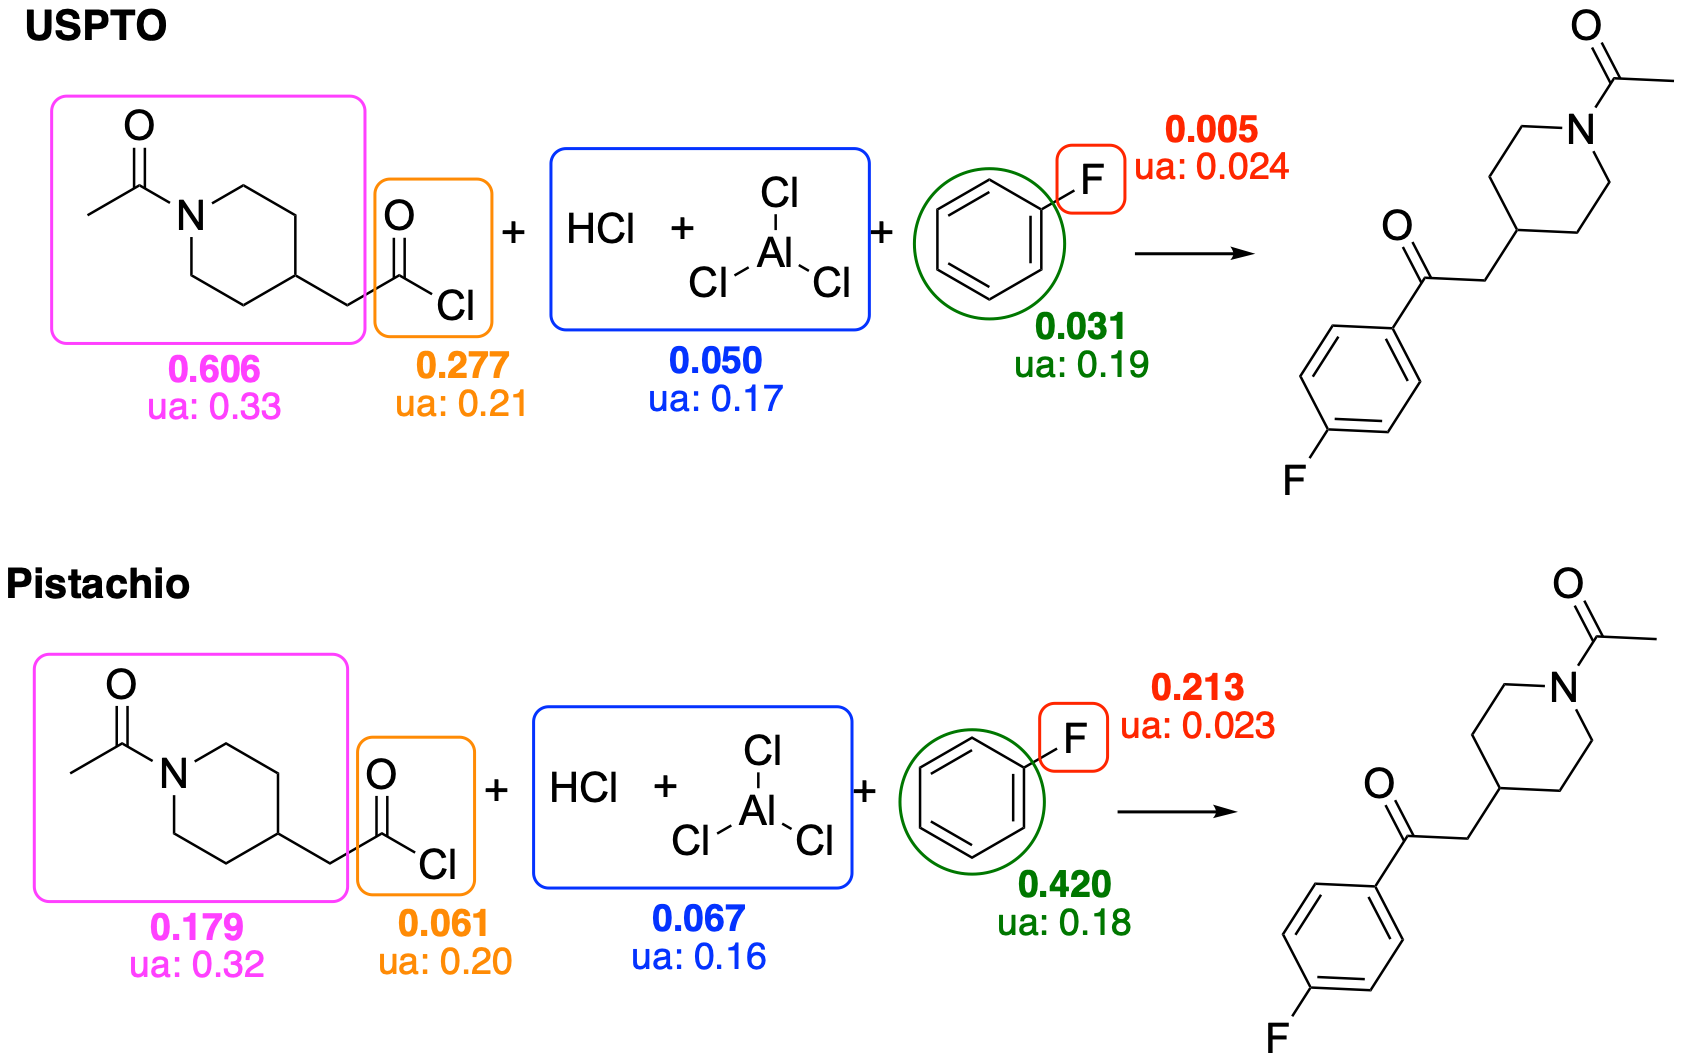
\includegraphics[width=0.8\textwidth]{Chapter4/Figs/sear_pred.png}
\caption[FC IG]{Both models predict the correct Friedel-Crafts acylation product but only the Pistachio model recognizes the importance of the -F atom in determining selectivity. The Integrated Gradients attributions are also shown along with the uniform attribution (ua) values. }
\label{fig:sear_pred}
\end{figure}

The predictions of the two models are shown in Fig~\ref{fig:sear_pred}. Both models predict the para selectivity correctly with confidence scores close to 1.0. When inspecting the IG attributions it can be seen that the USPTO model puts a very small weight on the Fluorine, only a fifth of the uniform attribution value. There is a large attribution given to the reagent though which does not affect the selectivity of this reaction at all. The attributions indicate that the USPTO transformer has not learnt the importance of F as the cause of para selectivity in these reactions. On the other hand the Pistachio transformer assigns a very high attribution value to F, suggesting that it has recognized the reason for the selectivity. 

Guided by the attributions we designed a number of adversarial examples where we have changed only the Fluorine part of the reactant-reagent input. This choice was motivated by the fact that according to the USPTO model the selectivity was driven by the reagents instead of the substituent on the benzene ring. If our interpretation is correct the model should keep predicting the para product even if a meta directing substituent is attached to the ring. The predictions of the models and the IG attributions of the meta directing groups are shown in Fig~\ref{fig:sear_adv}.

\begin{figure}[htbp!] 
\centering    
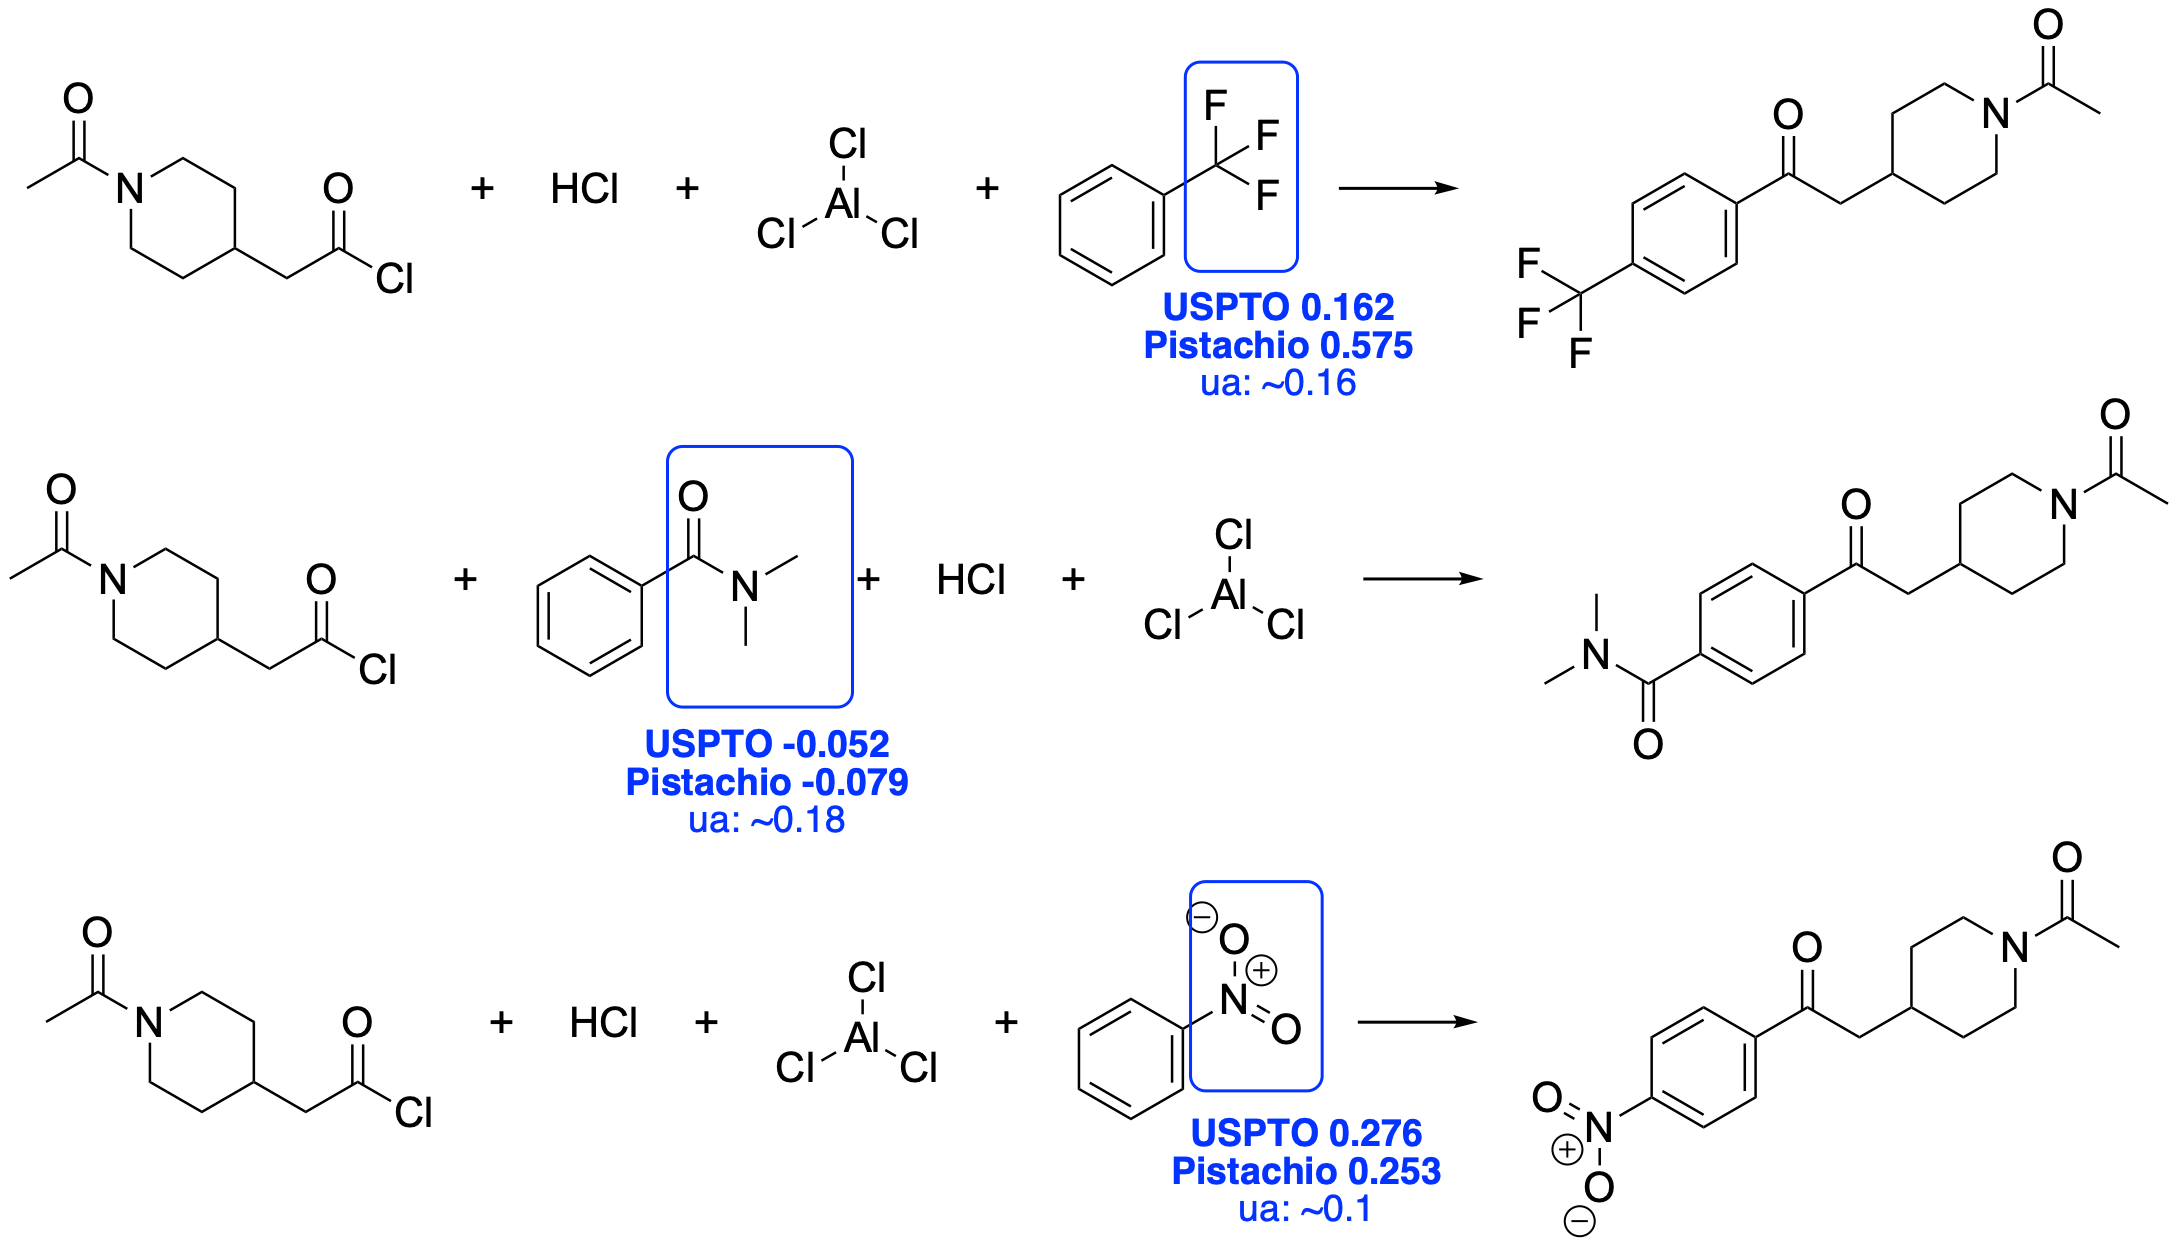
\includegraphics[width=1.0\textwidth]{Chapter4/Figs/sear_adv.png}
\caption[FC IG]{Adversarial examples designed using Fig~\ref{fig:sear_pred} reveal that both models can easily fail to predict the correct meta product. The uniform attribution (ua) values for the IGs are also shown. }
\label{fig:sear_adv}
\end{figure}

It can be seen that both transformer models fail in terms of predicting the meta directing effect of the substituents on the rings. In this case negative attributions favour the meta and positive the para product. There seems to be no correlation between the attribution values and the directing effect of the substituents, and even the Pistachio transformer is struggling with identifying the chemically important parts of the input. 

A suggestive observation is that in the second example the attributions on the meta directing group are negative, meaning that according to the models the amide group (correctly) favours the formation of the meta product. This agrees with chemical principles, but the model is still predicting the para to be the major product. We hypothesized that this might be due to biases in the training data, because if there are many more para substitution reactions than meta, the model could become biased towards predicting para substitutions even in the presence of meta directing groups. 

\begin{figure}[htbp!] 
\centering    
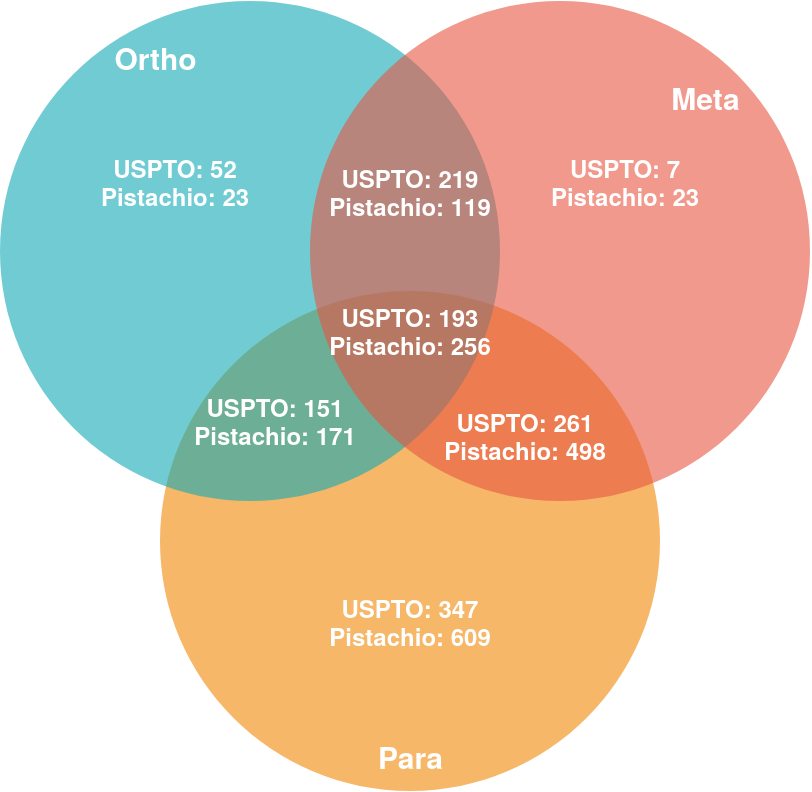
\includegraphics[width=0.65\textwidth]{Chapter4/Figs/sear_directing.png}
\caption[FC IG]{Counting the number Friedel-Crafts acylation reactions in the training sets with ortho, meta and para selectivities reveals an alarming bias -- the number of para reactions far outweigh those of meta or ortho reactions.}
\label{fig:sear_dir}
\end{figure}

To check if this hypothesis was correct we counted the number of ortho, meta and para Friedel-Crafts acylations in the training dataset using reaction templates. There was a large number of reactions matching multiple templates because often the benzene rings had multiple substituents on them. The results are summarized on Fig~\ref{fig:sear_dir}. 

The overall number of meta substitutions was 680 and 896 for the USPTO and Pistachio datasets respectively compared to the 952 and 1534 para substitutions. However, these numbers do not reveal the true extent of the bias as in our test case the benzene ring was only singly substituted. The number of reactions where there is only a single meta directing group on the ring is only 7 and 23 for the two datasets, which are extremely small numbers compared to those for a single para directing substituent which are 347 and 609, a ratio of 25-50 times.

This may result in the models not being able to learn meta directing substitution reactions because it can already achieve very high (~98\%) accuracy on the training set by always predicting the para product. The inclusion of further meta substitution reactions could considerably increase the models performance in real tasks. To confirm that the model would be able to learn the selectivities if the dataset was not biased, we probe the model with a synthetic dataset of para and meta Friedel-Crafts reactions in Sec.~\ref{subsec:synth_data}.

\subsection{Selective reduction of aldehydes and ketones}
Reduction of esters and aldehydes follow very well defined selectivity that is determined by the reducing agent. It is possible to reduce selectively an aldehyde or a ketone to alcohol in the presence of an ester. In this example the reduction of aldehydes using sodium-borohydride is examined \cite{Clayden2012}. If the Na is replaced by Li the reduction stops being selective to aldehydes and esters get reduced as well. The question is whether the models were able to learn the role of the cations in driving this subtle selectivity. An example reaction containing this selectivity is shown in Fig~\ref{fig:redu}.

\begin{figure}[htbp!] 
\centering    

\includegraphics[width=0.9\textwidth]{Chapter4/Figs/reduction.png}
\caption{An example of a reaction showing how NaBH\textsubscript{4} reduces the aldehydes selectively in the presence of an ester.}
\label{fig:redu}
\end{figure}

Both models are able to predict the product correctly with very high confidence (score > 0.95). In this case it is not immediately obvious what an interpretable attribution would be. One could argue that the selectivity is caused by Na\textsuperscript{+} because if we swap it to Li\textsuperscript{+} the other product would become the true product. The IG attributions on the \texttt{[Na+]} token are 0.013 and 0.017 for the USPTO and Pistachio models respectively, less than what the uniform attribution would be. This suggests that the models have not identified the importance of Na\textsuperscript{+} ion. 

To better understand the reliability of the predictions we attribute the reaction to the training data. For both models the most similar reactions (Fig~\ref{fig:redu_dat}) are BH\textsubscript{4} reductions of molecules containing both a ketone and an ester group. These examples suggest that both models have learnt this selectivity correctly, but they are not helping in understanding the role of the Na\textsuperscript{+}ion in the reaction.

\begin{figure}[htbp!] 
\centering    

\includegraphics[width=0.9\textwidth]{Chapter4/Figs/reduction_dat.png}
\caption{Data attribution to the reaction in Fig~\ref{fig:redu} suggests that both models have correctly learnt the selectivity of reduction.}
\label{fig:redu_dat}
\end{figure}

To investigate further if the models have learnt the importance of the cation in these reactions we designed an adversarial example where the only difference from the reaction on Fig~\ref{fig:redu} was the replacement of Na\textsuperscript{+} with Li\textsuperscript{+}. From Fig~\ref{fig:redu_adv} we see that the USPTO transformer keeps predicting the aldehyde being selectively reduced whereas the Pistachio model recognizes the change and predicts the correct product with both groups reduced. 

\begin{figure}[htbp!] 
\centering    
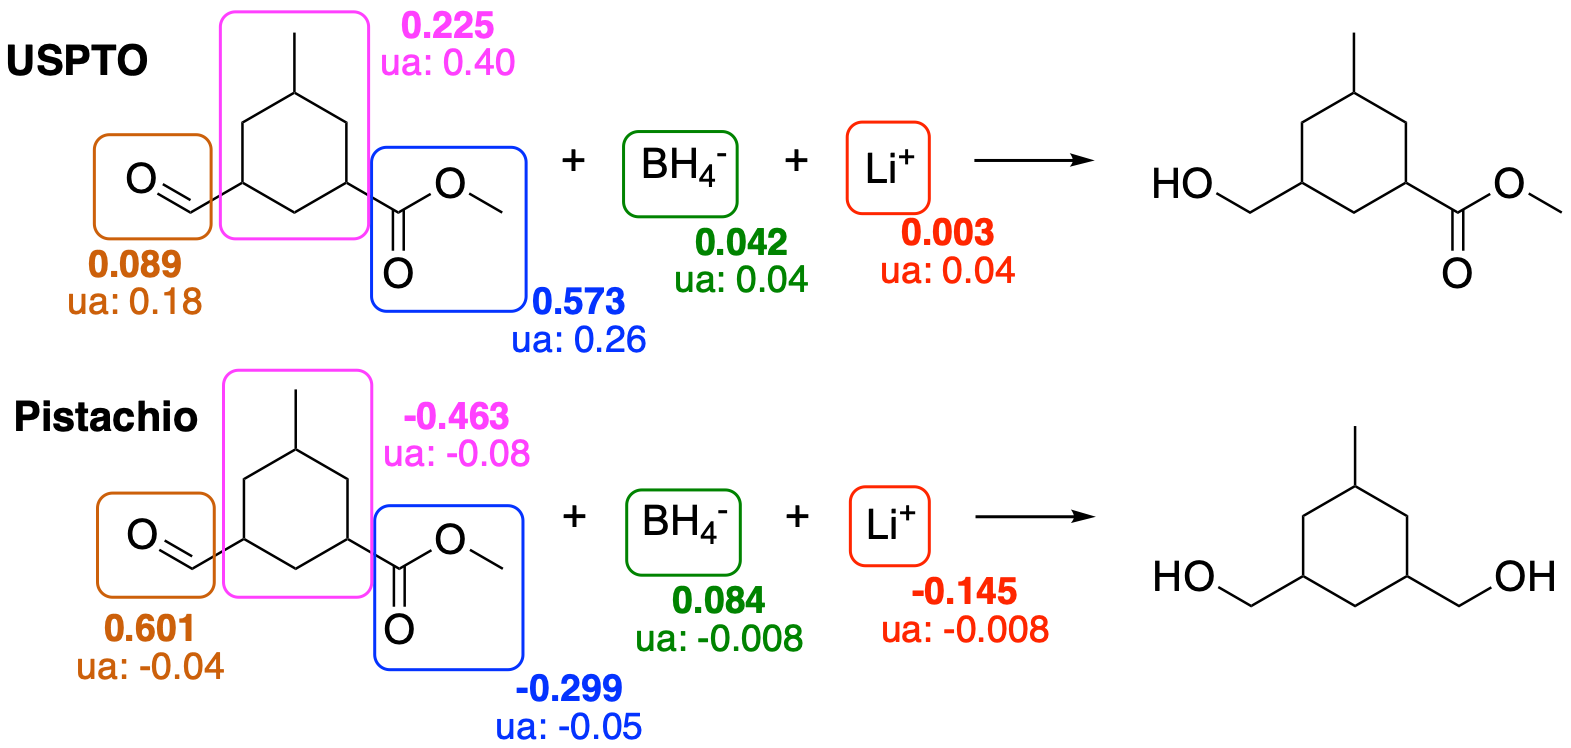
\includegraphics[width=0.9\textwidth]{Chapter4/Figs/redu_adv.png}
\caption{Adversarial example for the borohydride reduction in Fig~\ref{fig:redu} where the Na\textsuperscript{+} ion was replaced by Li\textsuperscript{+} ion. The USPTO model continues predicting the selective reduction of the aldehyde wrongly whereas the Pistachio model predicts the correct product -- the understanding of the models is reflecting in the IG attribution on the Li\textsuperscript{+} ion.}
\label{fig:redu_adv}
\end{figure}

To prove that one model was able to identify the importance of the cation and the other was not the IG attributions were generated and are shown in Fig~\ref{fig:redu_adv}. Here positive attributions favour the selective reduction, and the negative attributions favour the correct product. It is immediately obvious from the attributions that the USPTO model did not take into account the Li\textsuperscript{+} ion as it was given an attribution score that is an order of magnitude smaller than the uniform attribution value.

For the Pistachio model the probability score difference between the products was -0.21 and there was a lot of variation in attribution across different parts of the structure. The \texttt{[Li+]} token was given a very large negative attribution meaning that the model was strongly relying on it when making the correct prediction. Overall comparing the attributions it can be concluded that the USPTO model did not learn the chemistry of LiBH\textsubscript{4}, but the Pistachio one did. This can be due to the fact that the Pistachio model has seen more than 6 times more examples with this reagent. 

\subsection{Exploring the model with artificial data}
\label{subsec:synth_data}
One of the limitations of learning chemistry from patented and published reactions is that these reactions were designed by trained chemists who avoid transformations that have non-obvious selectivities. This makes it difficult for the models to infer the order of reactivity of functional groups. A further point is the effect of bias in the datasets on the models performance. To better understand these effect with full control over the experimental parameters, we have designed two artificial tasks where the training reaction data is generated using explicit SMARTS templates. 

In the first experiment we test whether the transformer model is able to learn selective chemistry if given enough data. We assembled a synthetic dataset of 90 000 reduction reactions. Carbon scaffolds were randomly selected from the ZINC database of drug-like molecules \cite{Irwin2005ZINCScreening}. To each scaffold we added an aldehyde group, an ester group, or both. Finally the 90 000 reactions, summarized in Table~\ref{table:red_datasets}, were obtained by applying one of three reduction templates shown in Fig~\ref{fig:redu_templates} to them. 

\begin{figure}[htbp!] 
\centering    

\includegraphics[width=0.6\textwidth]{Chapter4/Figs/redu_templates.png}
\caption[epoxide IG]{Three uniquely selective reduction templates are chosen to challenge the transformer's ability to learn selectivities if given enough data.}
\label{fig:redu_templates}
\end{figure}

\begin{table}[!h]
\caption{Number of reactions in the synthetic reduction datasets}
\centering
\label{table:red_datasets}
\begin{tabular}{m{0.17\textwidth}>{\centering}m{0.1\textwidth}>{\centering \arraybackslash}m{0.1\textwidth}>{\centering \arraybackslash}m{0.1\textwidth}}
\toprule
 \textbf{Subset} & \textbf{Aldehyde} & \textbf{Ester} & \textbf{Both}\\ 
\midrule
NaBH\textsubscript{4} & 20 000 & 0 & 10 000  \\
DIBAL & 0 & 20 000 & 10 000  \\
LiAlH\textsubscript{4} & 10 000 & 10 000 & 10 000  \\
\bottomrule
\end{tabular}
\end{table}

When training the transformer on this dataset we found that the only limiting factor in the performance of the model was its ability to reconstruct the sometimes tricky backbones of the molecules from the ZINC dataset. The selective chemistry was learnt (99\% top-1 accuracy) by the model in less than 10 000 steps. This shows that given sufficient data the model is able to learn selective transformations. To investigate how these findings are reflected in the IG attributions and verify that they are able to capture these empirical observations we generated the attributions for the reaction shown in Fig~\ref{fig:toy_attr}.

\begin{figure}[htbp!] 
\centering    
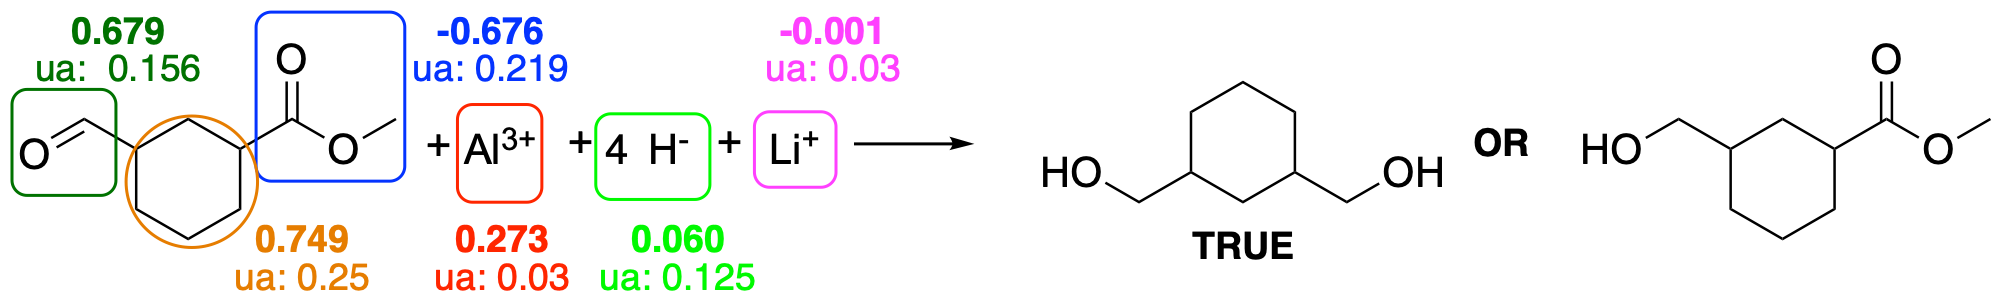
\includegraphics[width=1.00\textwidth]{Chapter4/Figs/toy_attr.png}
\caption{The model trained on artificial reduction data correctly attributes importance to the Al\textsuperscript{3+} ion.}
\label{fig:toy_attr}
\end{figure}

From the attributions we see that the model rightly gives high attribution to the Al\textsuperscript{3+} ion and small attribution to Li\textsuperscript{+}. This suggests that the model has learnt that it should only attend to one of the two tokens because they always appear together in the reactions. The H\textsuperscript{-} ions get a low attribution as expected. The attributions also verify that the model is finding the backbone part of the input very important, as reconstruction of the backbone is the most challenging aspect of making a correct prediction for this dataset of diverse backbones but restricted chemistry.

In the second more challenging synthetic experiment we investigated the models ability to learn the selectivity of aromatic electrophilic substitution reactions. By constructing balanced and biased datasets of Friedel-Crafts acylation reactions we hope to recover the observed behaviour in Sec.~\ref{subsec:friedel}. In the balanced and biased datasets we chose 10 para and 10 meta directing substituents which were placed on a benzene ring. For the last `super-biased' dataset, we only included three of the 10 meta directing substituents. These made the initial set of 20 reactant molecules which were reacted with a set of acyl chlorides generated by enumerating all possible straight carbon chains up to 8 carbons with a maximum of one double bond. This way we obtained 310 acyl chlorides that were reacted with the substituted benzenes to yield the meta or the para product. We use small carbon chains rather than the ZINC scaffolds to facilitate the learning of the backbones compared to learning the chemistry, which is partly why the dataset size was reduced as well and SMILES augmentation was applied. A summary of the training sets is shown in Table~\ref{table:synth_datasets}.

\begin{table}[!h]
\caption{Number of reactions in the synthetic Friedel-Crafts training datasets}
\centering
\label{table:synth_datasets}
\begin{tabular}{m{0.17\textwidth}>{\centering}m{0.1\textwidth}>{\centering \arraybackslash}m{0.1\textwidth}}
\toprule
  & \textbf{Meta} & \textbf{Para} \\ 
\midrule
Balanced & 3100 & 3100  \\
Biased & 310 & 2790  \\
Super-Biased & 30 & 3000  \\
\bottomrule
\end{tabular}
\end{table}

The USPTO and Pistachio transformers were trained for $\sim$300 and $\sim$100 epochs respectively, so this is the regime we wanted to investigate. We trained 10 transformer models on each of the datasets and saved checkpoints regularly. We created a test set using three meta directing and three para directing substituted benzenes combined with acyl chlorides not in the training sets, resulting in a balanced test set made up of 177 meta and 177 para substitution reactions. Using SMARTS template matching, we tested what proportion of the model predictions (with valid SMILES) are meta and para as a function of the number of epochs for different dataset biases. The results are shown in Fig~\ref{fig:synth_conv}. 

\begin{figure}[htbp!] 
\centering    
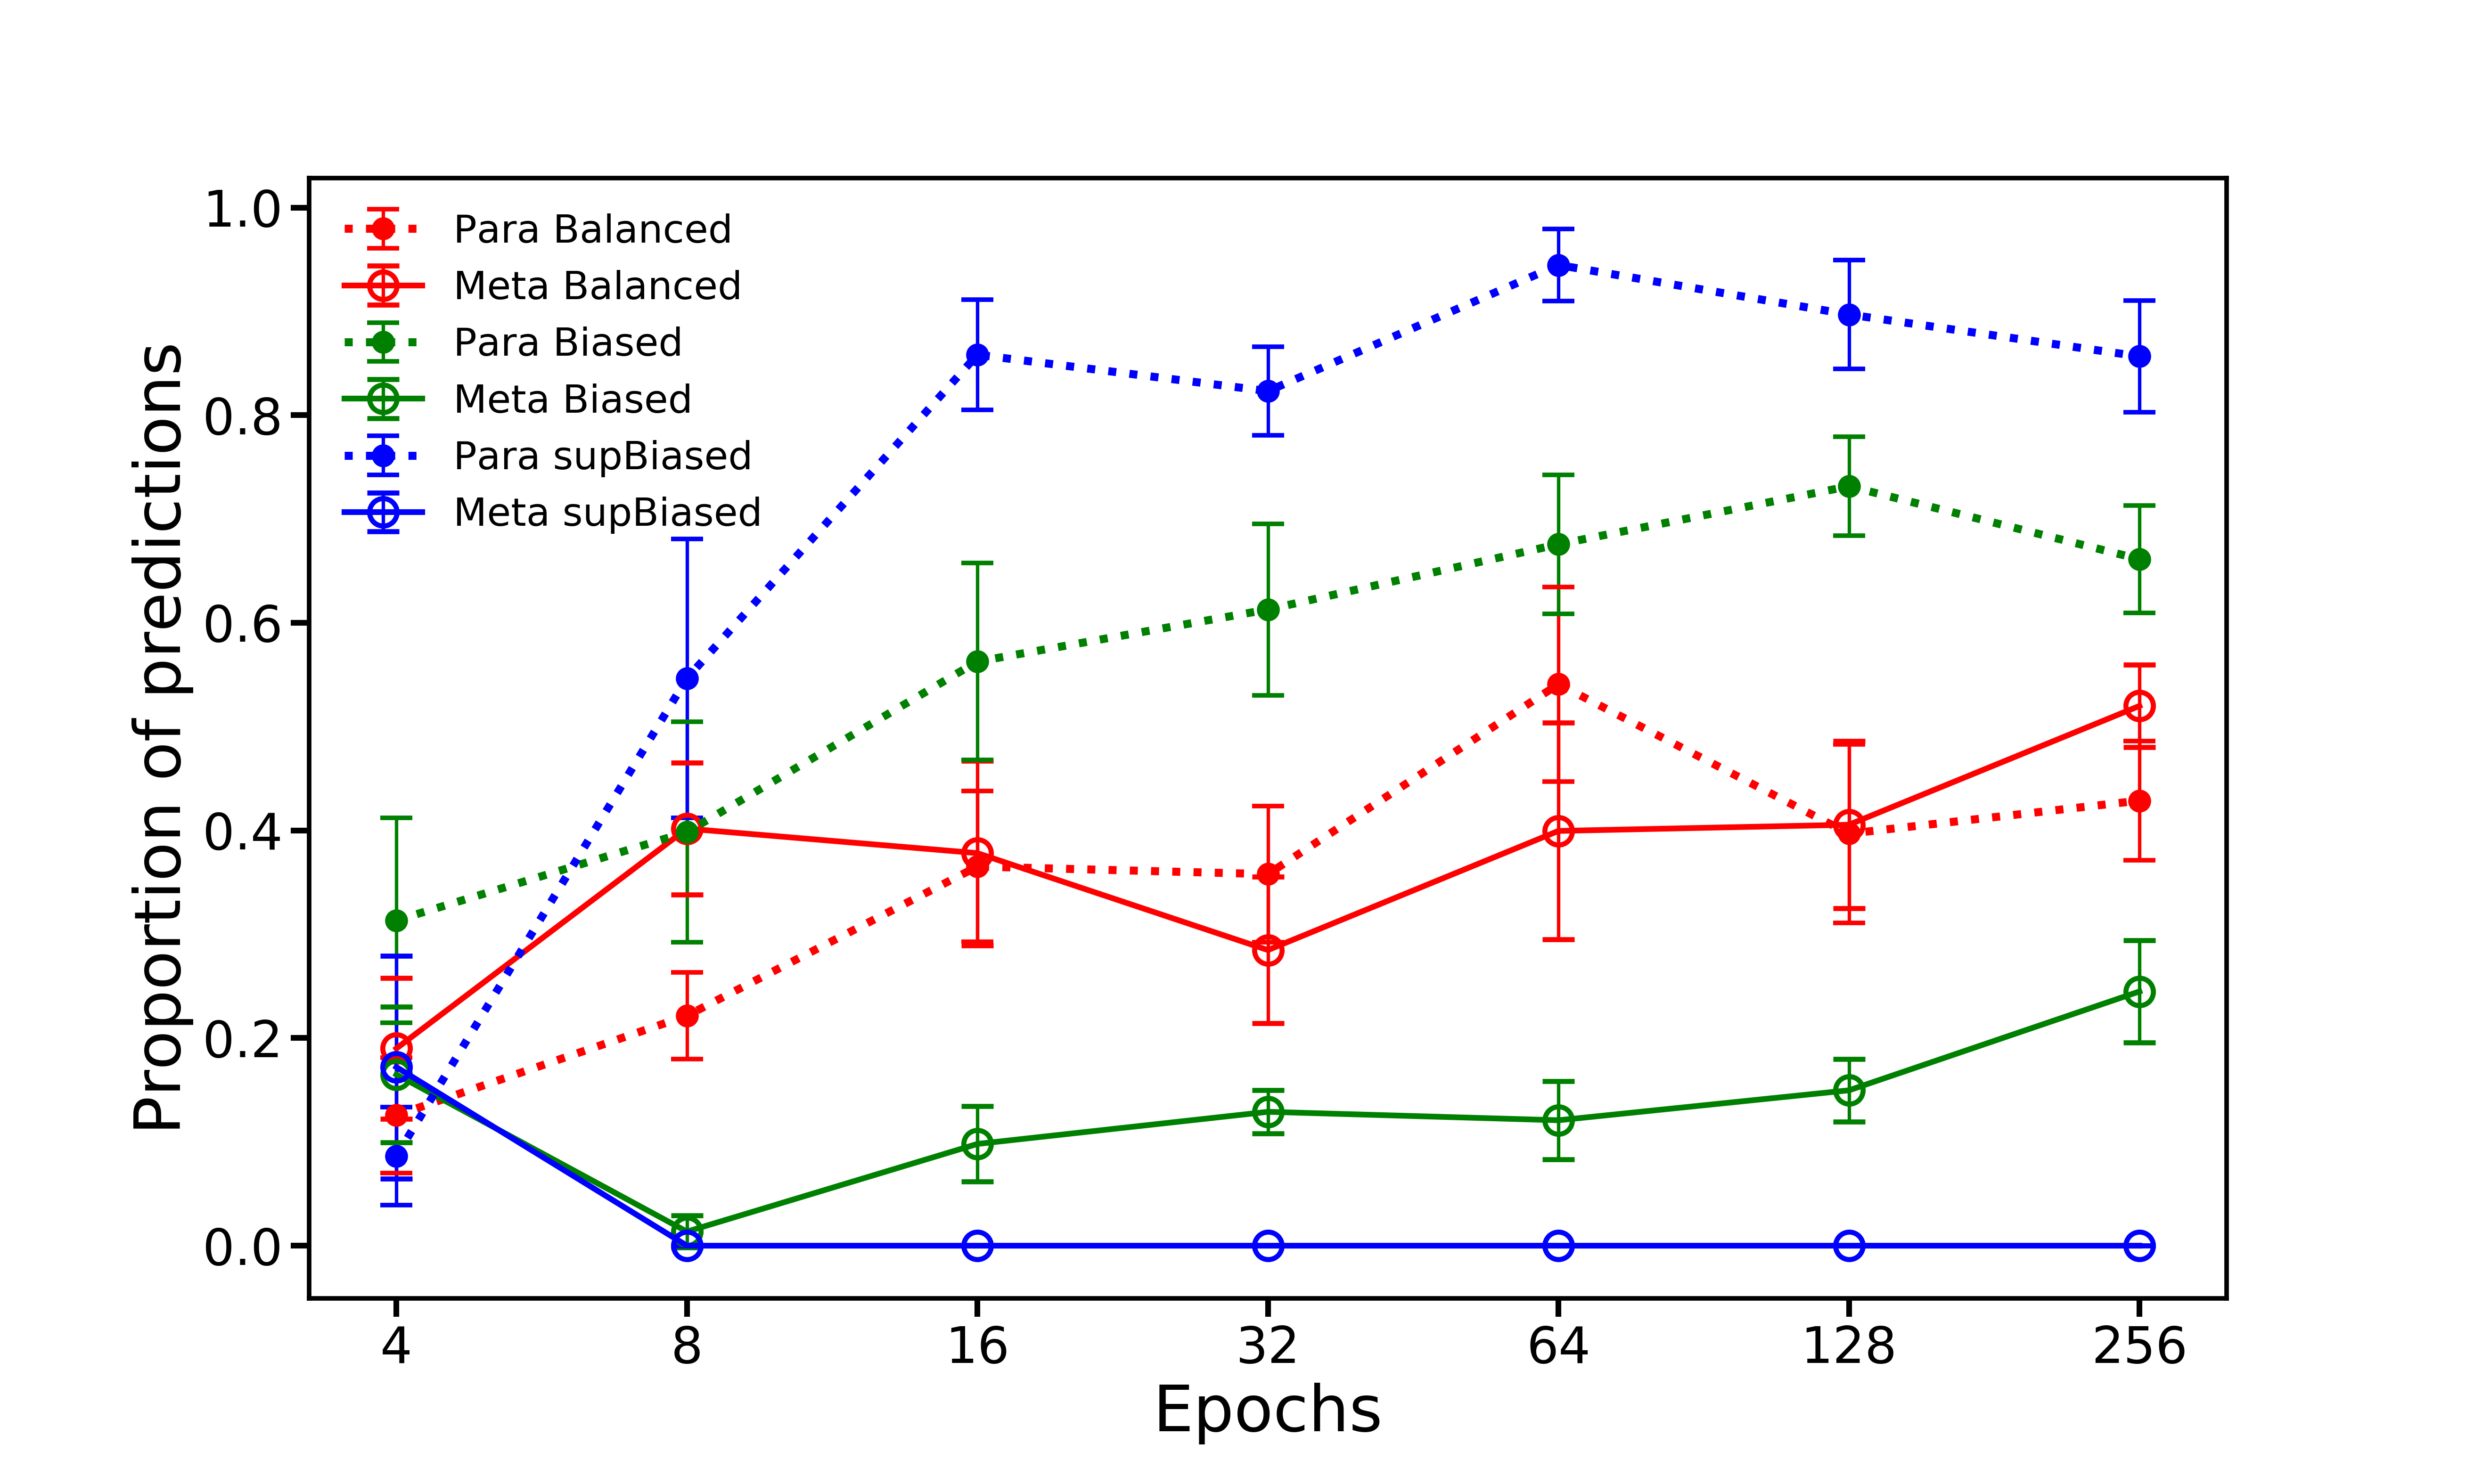
\includegraphics[width=1.0\textwidth]{Chapter4/Figs/synth_conv.png}
\caption{Dataset bias is reflected in the model predictions. The figure shows the proportion of para (solid line) and meta (dashed line) predictions on a balanced test set as a function of the number of training epochs for different biased training sets. }
\label{fig:synth_conv}
\end{figure}

We see that the balanced dataset converges quickly close to the correct ratio of 1:1 between meta and para predictions. On the other hand the bias in the training set is reflected in the predictions of the other two models, in the case of the super-biased model to the extent that it does not predict any meta products. This is particularly revealing because that is the training set whose ratio is closest to that found in the USPTO and Pistachio datasets. This serves as empirical proof that the observed failure to predict the meta substituent in Sec.~\ref{subsec:friedel} is the result of biases in the dataset. 

Finally we ran the models to convergence to see if eventually they are able to predict the correct structures. After $\sim$4 000 epochs the ratio of meta to para was exactly 1:1 for the balanced dataset and about 3:5 on both the biased and super-biased datasets. This shows that by training longer the effect of dataset bias can be mitigated, but it cannot be removed altogether. 

\subsection{Outlook}
\label{chap:conclusion}

Chemical reaction prediction models have undergone a revolution driven by innovations in the field of machine learning. This large increase in accuracy came at the expense of interpretability as expert crafted rules and reaction mechanisms gave way to black-box deep learning models. 

The predictions of machine learning models depend on two essential components. One of them is the training data which acts as an upper limit to the performance of the model. Any machine learning model can be only as good as the data it was trained on. The other ingredient is the input that is processed and turned into the prediction. We have developed two robust methods for interpreting and testing reaction prediction models focusing on each of these two ingredients, and applied them to analyse the Molecular Transformer which is the current state-of-the-art model. 

The first method builds on the Integrated Gradients method \cite{Sundararajan2017AxiomaticNetworks} for attributing the prediction of neural network models to parts of the input. This method has been used to identify which parts of the inputs to the model are important when predicting typical selective chemical reactions. It has been found that often the model does not identify chemically important substructures, demonstrated by the design of adversarial examples based on the attributions which fool the model.

The other method we developed attributes the predictions of the model to training data. We averaged the vector outputs from the last encoder layer of the Molecular Transformer to define a similarity metric between different reactions, as understood by the model. Attributing back to training data serves multiple purposes in the case of reaction prediction. It can either support or invalidate a prediction by telling the user which are the most similar training reactions according to the model. Furthermore this can be used to identify unknown trends or biases in the dataset or sometimes even to identify erroneous training examples. 

Using evidence from these attribution methods, we hypothesized that many of the erroneous predictions of the Molecular Transformer model stem from data biases. We have validated this hypothesis by designing an artificial dataset of Friedel-Crafts acylation reactions where we could show how biases in the dataset manifest in the predictions of the model. In addition, we observe that the model trained on the Pistachio dataset had in general better predictions and much better calibrated uncertainty scores, in spite of the fact that this model only achieved 76\% test-set accuracy. This suggests that Pistachio is not as biased as USPTO, and hints that the addition of training data can substantially improve model performance. 

From these results we believe that for reaction prediction, the Top-$N$ accuracy from testing on randomly chosen held-out test sets do not provide an adequate measure of the models true performance and generalization ability. We believe that this is partly results from the fact that publications and patents often contain reaction carried out on a series of analogous reactants. Therefore there is a high chance that essentially identical reactions end up in the training and test sets. A more honest measurement of the model's true generalizability could be realized by only including reactions in the test-set whose products have a low similarity to the products in the training set. The exploration of this idea is the subject of further work. 

Overall, from this work we believe that improvements to the training data can be just as impactful as improving the machine learning models themselves. By demonstrating the power of interpretability methods when rigorously applied to scientific questions, we have shown that these methods can be useful beyond just giving explanations of predictions by exposing dataset biases. Applying our approach for data and input interpretation beyond chemical reaction prediction to other fields will likely be equally constructive, illuminating the path to improved training data and hence improved artificial intelligence models.
\chapter{Augmenting Nanomolar High-Throughput Screening with Machine Learning for Lead Optimisation}

Typically, testing a drug candidate involves obtaining a pure sample of the molecule, and then mixing it in solution with the protein target under study to measure its bioactivity via an assay. While necessary for maximum accuracy, compound purification can be time-consuming and costly, particularly for chiral molecules. In collaboration with the London Lab at The Weizmann Institute of Science, we investigated whether we needed compound purification at all for training machine learning bioactivity models by using non-purified compound assays. Focusing on a particular scaffold synthesised with an amide coupling as the final step, we added the acid and amine reactants directly in solution with the protein to obtain an assay reading from the crude reaction mixture. By skipping the purification step, this allowed us to quickly screen a library of < 300 > amines with the same acid in high-throughput which we used to train RF and GP models. Leave-one-out validation on the training data correctly identified false negatives, and a prospective virtual screen of EnamineREAL with the trained models returned top hits with similar potency and better pharmacokinetic properties.

TODO - include figures
%!TEX root = ../thesis.tex
%*******************************************************************************
%****************************** Third Chapter **********************************
%*******************************************************************************
\chapter{Future Work}


\section{Short-Term: Continutation of ongoing work}
Given the relative success of work so far, the immediate plan is to continue ongoing research to completion. After developing a more appropriate benchmark dataset for evaluating the performance of reaction prediction models, the intention is to write up the results of chapter \ref{chap:MolTrans} within the next month, potentially following up with an attempt to `fix' the model which may also be a contribution to the field of NLP in particular regarding the modelling of long sequences. The investigation into SOAP descriptors for QSAR should hopefully be concluded shortly after resubmitting the results to JMedChem. If the drug candidates proposed by the Siamese GNN prove potent, then there is a strong incentive to refine and retrospectively validate the model on historical data and publish the methodology.

In addition, the COVID Moonshot project will likely continue for another $\sim$8 months and I will continue my participation of the project given the obvious urgency of the pandemic. No doubt this enterprise will remain a fruitful source of interesting problems with real experimental data, which will hopefully lead to innovative solutions. Research will probably be on continuing optimisation of existing molecular series, or searching for alternative backup series while the most promising series undergo \textit{in vivo} toxicity screening.

\section{Long-Term: Investigation of new modalities}
Although using artificial intelligence for optimising the small-molecule drug discovery process is undoubtedly a difficult task, there has been extensive interest from both academia and private industry with many breakthroughs having been made already. The field is maturing to the extent that ML algorithms are already beginning to become part of the commercial design-make-test workflow, such that the remaining challenges are arguably merely an engineering problem. 

The therapeutic space beyond small-molecules, however, is relatively unexplored territory for data-driven techniques. Applying machine learning to this area will likely present even more complex challenges, but the potential impact of developing new modalities far outweigh that of `just' improving small-molecule QSAR modelling. While the potential areas of research are numerous, thus far two topics of interest have been identified:

\begin{itemize}
    \item functionalisation of flexible biomolecules (glycans, peptides),
    \item understand/design self-assembled nanostructures for drug delivery.
\end{itemize}

Both of these topics involve structures that are larger and less well-understood by medicinal (bio)chemists because of their energetic/entropic complexity. This is a promising area where I could combine physics-based intuition for modelling interactions, as well as pragmatic ML for designing models that would be useful in a drug discovery setting.

While no ML in involved in the Test of design-make-test it is nonetheless vital to retain this part of the cycle for proper validation of ML drug discovery methods, for taking the important step from mere concept to real-life data-driven-drugs. Therefore there is an expectation that some form of experimental work will be carried out, likely alongside more experienced collaborators, in the latter stages (2\textsuperscript{nd}-3\textsuperscript{rd} year) of the PhD irrespective of the ultimate direction of research.

% ********************************** Back Matter *******************************
% Backmatter should be commented out, if you are using appendices after References
%\backmatter

% ********************************** Bibliography ******************************
\begin{spacing}{0.9}

% To use the conventional natbib style referencing
% Bibliography style previews: http://nodonn.tipido.net/bibstyle.php
% Reference styles: http://sites.stat.psu.edu/~surajit/present/bib.htm

\bibliographystyle{apalike}
% \bibliographystyle{unsrt} % Use for unsorted references  
% \bibliographystyle{plainnat} % use this to have URLs listed in References
\cleardoublepage
% TODO - get references working
\bibliography{References/references} % Path to your References.bib file


% If you would like to use BibLaTeX for your references, pass `custombib' as
% an option in the document class. The location of 'reference.bib' should be
% specified in the preamble.tex file in the custombib section.
% Comment out the lines related to natbib above and uncomment the following line.

%\printbibliography[heading=bibintoc, title={References}]


\end{spacing}

% ********************************** Appendices ********************************

\begin{appendices} % Using appendices environment for more functionality

% %!TEX root = ../thesis.tex
% ******************************* Thesis Appendix A ****************************
\chapter{Computational Details} \label{appendix:details}

\section{Docking against SARS-CoV-2} \label{appendix:docking}
All molecules synthesised by the COVID Moonshot Consortium were docked against structure x2908 reported by Diamond XChem \cite{Douangamath2020XChem}. We use the “Classic OEDocking” floe v0.7.2 as implemented in the Orion 2020.3.1 Academic Stack (OpenEye Scientific). Omega was used to enumerate conformations (and expand stereochemistry) with up to 500 conformations. FRED was used for docking in HYBRID mode using the x2908 bound ligand. The docked poses of the ligands were scored using the Chemgauss4 scoring function.

\section{Machine learning} \label{appendix:machine_learning}
\subsection{FRESCO} \label{appendix:fresco}
All data and code used for this work can be found in the GitHub repo \url{https://github.com/wjm41/frag-pcore-screen}. Supplementary figures and tables can be found in an accompanying file.

\subsection{Ranking model} \label{appendix:ranking}
Our training set, de novo design method and generated molecules are available on \url{https://github.com/wjm41/mpro-rank-gen}.

\subsection{Transformer model} \label{appendix:transformer}
The Molecular Transformer architecture used throughout this work is based on the model described in Schwaller et. al. \cite{Schwaller2019MolecularPrediction}. 

The model uses a 256 dimensional learnt embedding for each SMILES token. The encoder and the decoder are both made up of 4 standard transformer layers and dropout is applied with probability 0.1 \cite{Srivastava2014dropout}. For weight optimization the Adam optimizer is used and the model is trained for 500 000 steps. Checkpoints are saved every 10 000 steps and the final model is obtained by averaging the weights of the last 20 checkpoints for USPTO.

The model was implemented with OpenNMT-py package \cite{Klein2017} which makes use of the PyTorch framework \cite{paszke2019pytorch}. 

All code used for implementing the attribution tools for the Molecular Transformer, generating the artificial Friedel-Crafts dataset, and Tanimoto-splitting USPTO can be accessed in the GitHub repo \href{https://github.com/davkovacs/MTExplainer.git}{MTExplainer} \cite{Kovacs2020MolecularExplainer}. The USPTO dataset used to train the model \cite{Lowe2012, Jin2017}, as well as the Tanimoto similarity-based train/test splits of USPTO can also be found in the GitHub repo.
% %!TEX root = ../thesis.tex
% ******************************* Thesis Appendix B ********************************

\chapter{Experimental Details} \label{appendix:experiments}

\section{Mpro assay} \label{appendix:mpro_assay}
The experimental procedure for measuring Mpro inhibition via Homogeneous Time Resolved Fluorescence (HTRF) assay is the same as that previously reported by COVID Moonshot\cite{Moonshot2022}, which is repeated below.

Dose response assays were performed in 12 point dilutions of 2-fold, typically beginning at 100\uM. Highly active compounds were repeated in a similar fashion at lower concentrations beginning at 10\uM or 1\uM. Reagents for Mpro assay were dispensed into the assay plate in 10$\mu$l volumes for a final volume of 20$\mu$L.

Final reaction concentrations were 20mM HEPES pH7.3, 1.0mM TCEP, 50mM NaCl, 0.01\% Tween-20, 10\% glycerol, 5nM Mpro, 37nM fluorogenic peptide sybstrate ([5-FAM]-AVLQSGFR-[Lys(Dabcyl)]-K-amide). Mpro was pre-incubated for 15 minutes at room temperature with compound before addition of substrate and ex/em filter set. Raw data was mapped and normalized to high (Protease with DMSO) and low (No Protease) controls using Genedata Screener software. Normalized data was then uploaded to CDD Vault (Collaborative Drug Discovery). Dose response curves were generated for IC50 using nonlinear regression with the Levenberg-Marquardt algorithm with minimum inhibition = 0\% and maximum inhibition = 100\%.

\section{OC43 antiviral assay} \label{appendix:oc43_assay}
A549 expressing H2B-mRuby were seeded in 384 well plates (4,000 cells per well) in DMEM+2\% FCS in a total volume of 30ul. One day later, 20ul of OC43 were added to the wells for a final MOI of 0.3. one hour after viral addition, the drug (or DMSO as control) was added to the cells. Drugs were added at a volume of 50nl, in a final dose range of 0.3-20mM. Cells were incubated at 33C, 5\% CO2 for 2 days, fixed with paraformaldehyde and stained for the presence of the viral nucleoprotein. Images were captured and quantified using the Incucyte machine and software. 3 biological repeated were performed.

\section{Model generated reaction schemes} \label{appendix:rxn_schemes}
\begin{figure}
    \centering
        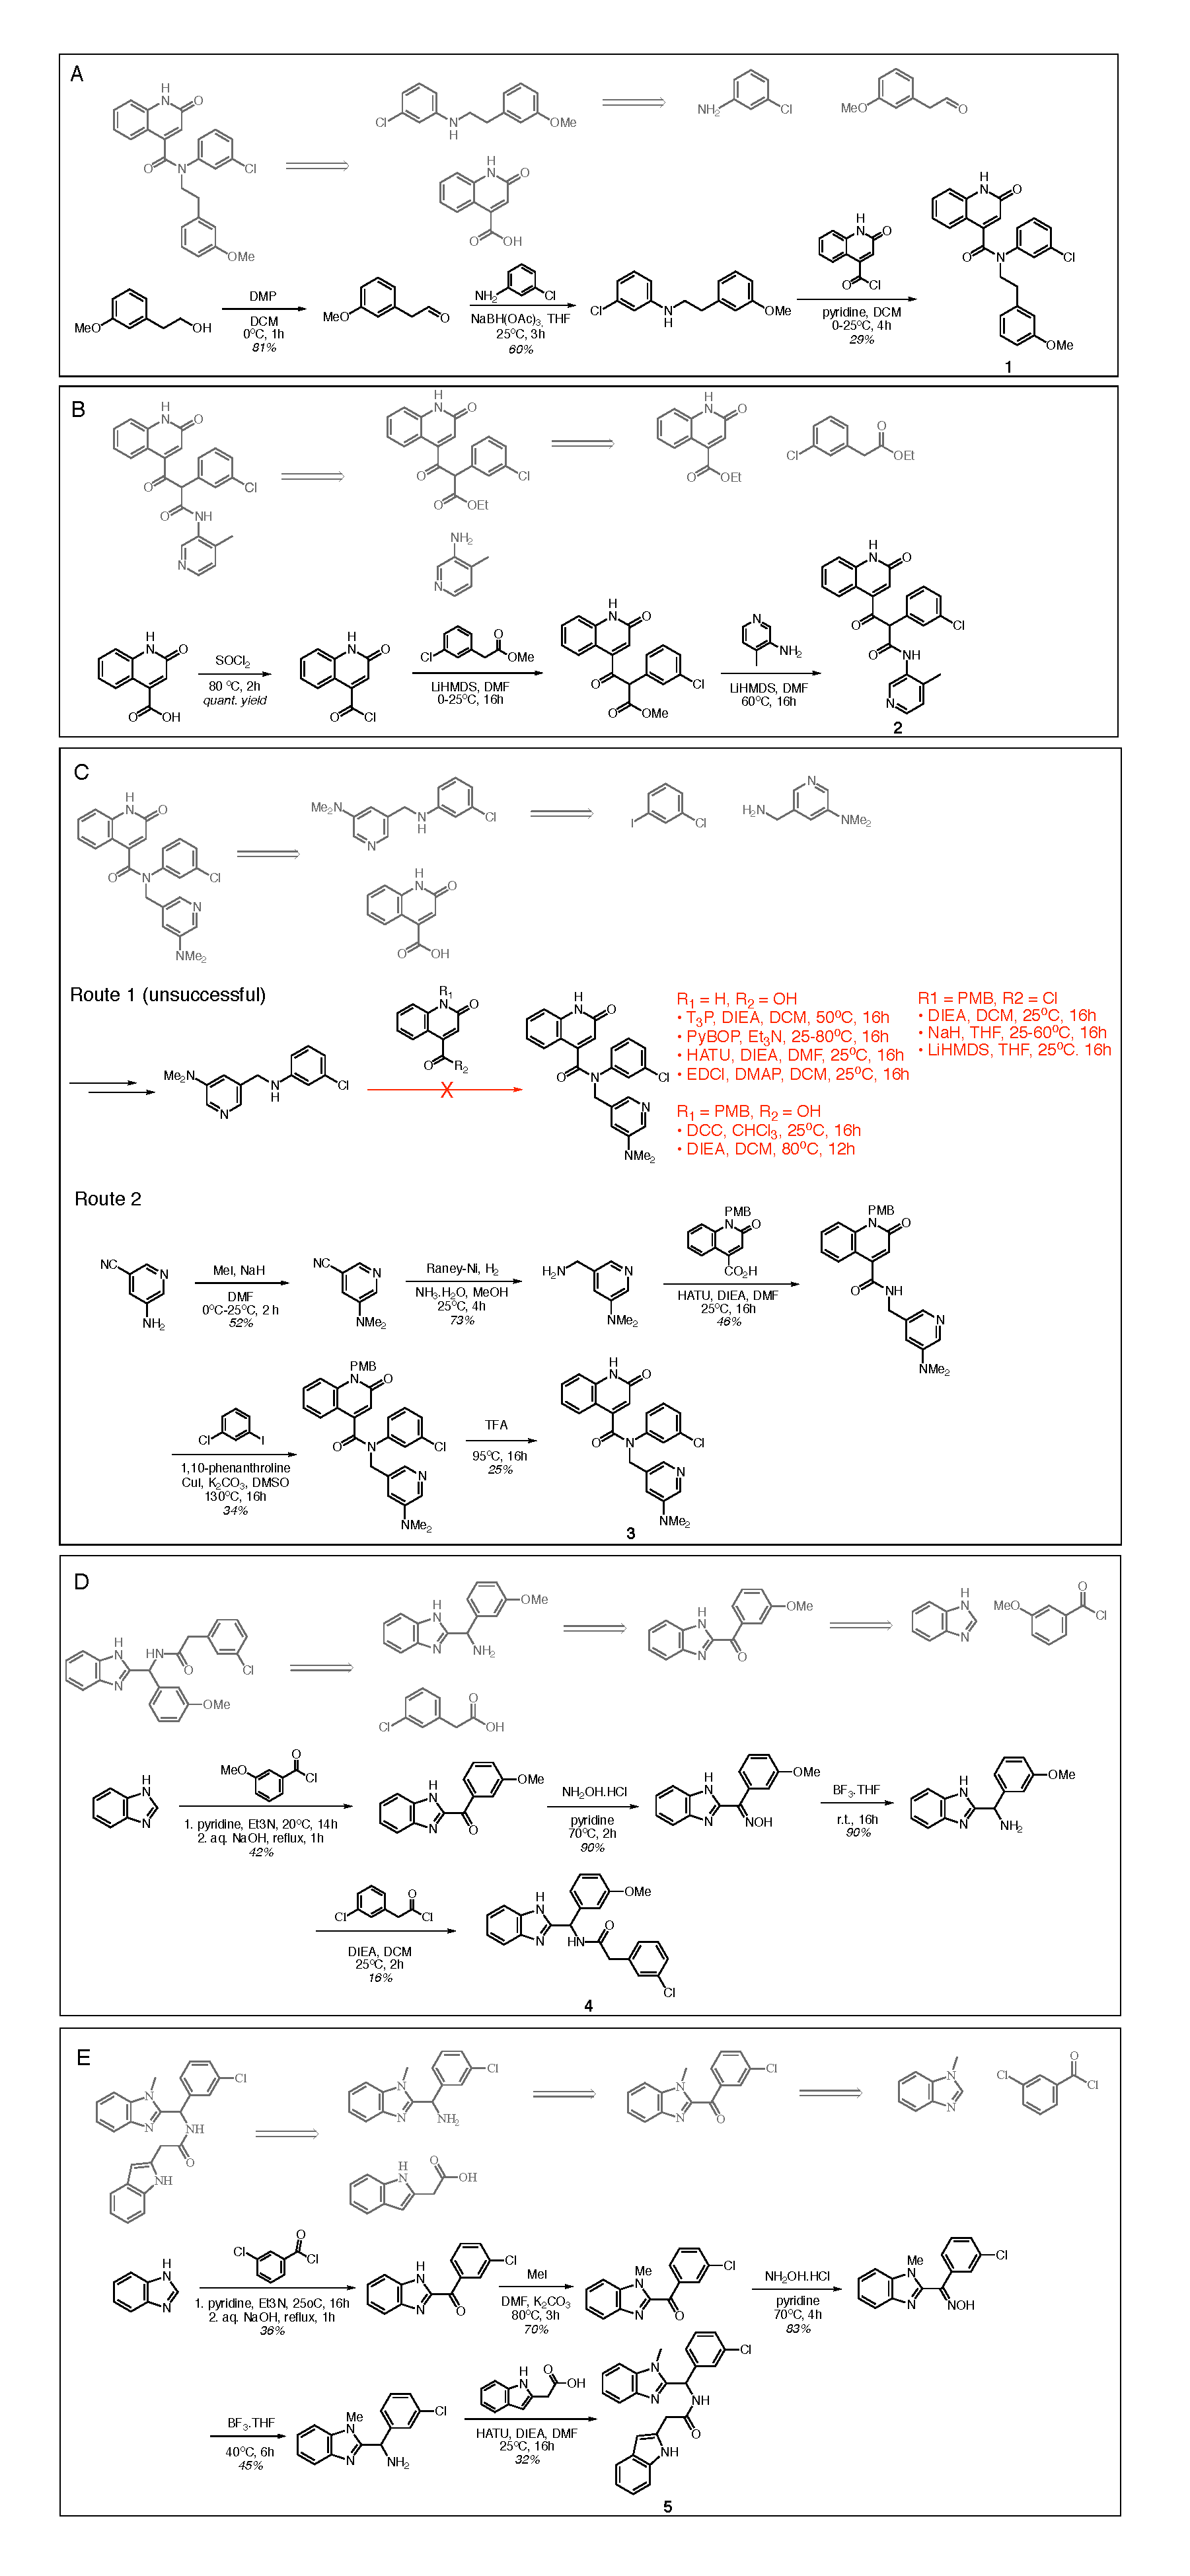
\includegraphics[width=0.6\textwidth]{Chapters/Ranking/Figs/rxn_schemes_full.pdf}
        \caption{Model generated synthetic schemes for compounds $\mathbf{1}$-$\mathbf{5}$. The synthesis schemes generated by our model (grey) and the experimental schemes (black).}
        \label{fig:appendix_synthesis_schemes}
\end{figure}

\section{Mac1 assay} \label{appendix:mac1_assay}
Inhibition of SARS-CoV-2 nsp3-Mac1 (aa residues 206–379 of nsp3) was assessed by the displacement of an ADP-ribose conjugated biotin peptide from His6-tagged protein using a HTRF-technology-based screening assay which was performed as previously described \cite{Schuller2021Mac1Frag}. Compounds were dispensed into ProxiPlate-384 Plus (PerkinElmer) assay plates using an Echo 525 liquid handler (Labcyte). Binding assays were conducted in a final volume of 16 $\mu$l with 12.5 nM SARS-CoV-2 nsp3-Mac1 protein, 400 nM peptide ARTK(Bio)QTARK(Aoa-RADP)S (Cambridge Peptides), 1:20000 Anti-His6-Eu3+ cryptate (HTRF donor, PerkinElmer) and 1:125 Streptavidin-XL665 (HTRF acceptor, PerkinElmer) in assay buffer (25 mM HEPES pH 7.0, 20 mM NaCl, 0.05\% bovine serum albumin and 0.05\% Tween-20). Assay reagents were dispensed manually into plates using a multichannel pipette while macrodomain protein and peptide were first dispensed and incubated for 30 min at room temperature. This was followed by addition of the HTRF reagents and incubation at room temperature for 1 h. Fluorescence was measured using a PHERAstar microplate reader (BMG) using the HTRF module with dual emission protocol (A = excitation of 320 nm, emission of 665 nm, and B = excitation of 320 nm, emission of 620 nm). Raw data were processed to give an HTRF ratio (channel A/B $\times$ 10,000), which was used to generate IC50 curves. The IC50 values were determined by nonlinear regression using GraphPad Prism v.9 (GraphPad Software, CA, USA).

\section{Crystallographic screening on SARS-CoV-2 nsp3-Mac1} \label{appendix:mac1_crystallography}
Crystallographic screening of compounds was performed using Mac1 crystals grown in the P43 space group, following the previously described protocol (PMID: 33853786). Compounds synthesized by Enamine/WuXi were prepared in DMSO to 100 mM and were added to crystallization drops using an Echo 650 liquid handler (Labcyte) (PMID: 28291760). Crystals were soaked at either 10 or 20 mM for 2-4.5 hours, before being vitrified in liquid nitrogen using a Nanuq cryocooling device (Mitegen). Soak times and concentrations are listed in Table S1. Diffraction data were collected at beamlines 12-1 and 12-2 of the Stanford Synchrotron Radiation Lightsource (SSRL). The data collection strategy and statistics are listed in Table S1. Compound binding was detected using the PanDDA algorithm (PMID: 28436492) as described previously (PMID: 35794891). PanDDA was initially run using a background map calculated with 34 datasets collected from crystals soaked only in DMSO (annotated as dmso\_34 in Table S1). PanDDA was rerun with a background map calculated using two sets of 35 datasets where no compound binding was detected (annotated as either ssrl\_1 or ssrl\_2 in Table S1). This procedure led to the identification of an additional nine hits (Table S1). 

Compounds were modeled into PanDDA event maps using COOT (PMID: 20383002) with coordinates and restraints generated by phenix.elbow from SMILES strings (PMID: 19770504). Duplicate soaks were performed for most compounds: where the same compound was identified in multiple datasets, the highest occupancy compound was modeled. Both the compound-bound and compound-free coordinates were refined together as a multi-state model following the protocol described previously (PMID: 28436492). Compound occupancy was set based on the background density correction (BDC) value (PMID: 28436492). Refinement statistics are presented in Table S1. Coordinates and structure factor amplitudes have been deposited in the protein data bank (PDB) with the group deposition code G\_1002254. PanDDA input and output files have been uploaded to Zenodo (DOI: 10.5281/zenodo.7231822), and the raw diffraction images are available at https://proteindiffraction.org/.

\section{High-Throuhput Amide Coupling} \label{appendix:amide_coupling}
The amide library was made by reacting the carboxylic acid under the optimized reaction conditions (2 eq. amine; 2 eq. EDC; 2 eq. HOAt; 5 eq. DIPEA; DMSO; RT; 24h) with 300 amines (202 aromatics, 49 primary, and 49 secondary aliphatic amines). For library production, we used Echo LDV plates and an Echo 555 acoustic dispenser for liquid handling. Plate copies were made after diluting the reaction mixture with 4 μL DMSO. For yield estimation, 1 μL of the diluted library was transferred to an LC/MS-ready 384-well plate, followed by dilution with 20\% ACN in water to the final volume of 50 μL. The desired product was identified in 60\% of wells.

\end{appendices}

% *************************************** Index ********************************
\printthesisindex % If index is present

\end{document}
